\chapter{Material}
\section{Sustainability and Steel Structures}
The issue of sustainability is becoming important in both NZ and worldwide policy and its consideration will affect choices made in the future.

The World Commission on Environment and Development in their 1986 report `Our Common Future' called for: \textit{a form of sustainable development which meet the needs of the present without compromising the needs of future generations to meet their own needs}.

Sustainability is commonly measured by the triple bottom line --- social, economic, and environmental priorities. For buildings, this is important because:
\begin{itemize}
\item social
\begin{itemize}
\item we spend about \SI{90}{\percent} of our time in buildings,
\item buildings affect our life quality,
\end{itemize}
\item economic
\begin{itemize}
\item buildings affect our productivity,
\item construction is about \SI{10}{\percent} GDP and employs many people,
\end{itemize}
\item environmental
\begin{itemize}
\item construction consumes many resources,
\item about one half of all energy is consumed in buildings,
\item construction and demolition generate huge amounts of waste each year.
\end{itemize}
\end{itemize}

Life cycle assessment (LCA) is a tool commonly used to assess environmental impacts of the built environment. The UK Building Research Establishment (BRE) has developed an environmental assessment methodology (EAM) for structures (BREEAM). A typical energy life cycle is given (from SSC) in \figref{fig:life_cycle}.
\begin{figure}[H]
\centering
\footnotesize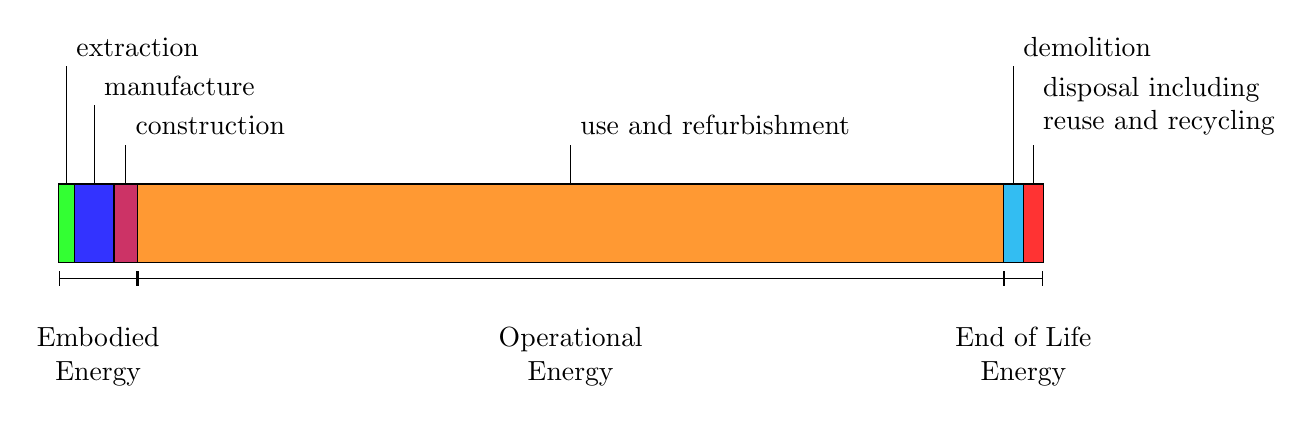
\begin{tikzpicture}
\def\a{.2}
\def\b{.7}
\def\c{1}
\def\d{12}
\def\e{12.25}
\def\f{12.5}
\draw(\a/2,1)--+(0,1.5)node[fill=white,anchor=south west]{extraction};
\draw(\a/2+\b/2,1)--+(0,1)node[fill=white,anchor=south west]{manufacture};
\draw(\b/2+\c/2,1)--+(0,.5)node[fill=white,anchor=south west]{construction};
\draw(\c/2+\d/2,1)--+(0,.5)node[fill=white,anchor=south west]{use and refurbishment};
\draw(\d/2+\e/2,1)--+(0,1.5)node[fill=white,anchor=south west]{demolition};
\draw(\e/2+\f/2,1)--+(0,.5)node[fill=white,anchor=south west,align=left]{disposal including\\reuse and recycling};
\draw[fill=green!80](0,0)rectangle(\a,1);
\draw[fill=blue!80](\a,0)rectangle(\b,1);
\draw[fill=purple!80](\b,0)rectangle(\c,1);
\draw[fill=orange!80](\c,0)rectangle(\d,1);
\draw[fill=cyan!80](\d,0)rectangle(\e,1);
\draw[fill=red!80](\e,0)rectangle(\f,1);
\draw[|-|](0,-.2)--(\c,-.2)node[below=.5cm,align=center,midway]{Embodied\\Energy};
\draw[|-|](\c,-.2)--(\d,-.2)node[below=.5cm,align=center,midway]{Operational\\Energy};
\draw[|-|](\d,-.2)--(\f,-.2)node[below=.5cm,align=center,midway]{End of Life\\Energy};
\end{tikzpicture}
\caption{Energy life cycle for an office building over \num{60} years}\label{fig:life_cycle}
\end{figure}

It may be seen that the embodied energy of the structure is only a small part of the total cost and that operational energy is the most significant. Embodied energy and end-of-life energy effects are minimized in structures with long lives.

Greater energy efficiency in buildings is generally achieved by a combination of the following measures:
\begin{itemize}
\item reducing primary heat losses through the building envelope, and cooling loads,
\item introducing energy saving measures in the operation of the building, e.g., energy efficient electrical appliances,
\item installing energy creation systems, such as photovoltaic panels and combined heat and power plants
\item improving natural lighting.
\end{itemize}

In the future, it is expected that structures will be built using not only one material, but a combination of materials. The REI Flagship store (Seattle)\footnote{\url{https://www.rei.com/stores/seattle.html}} is a good example of this.

\begin{figure}[H]
\centering
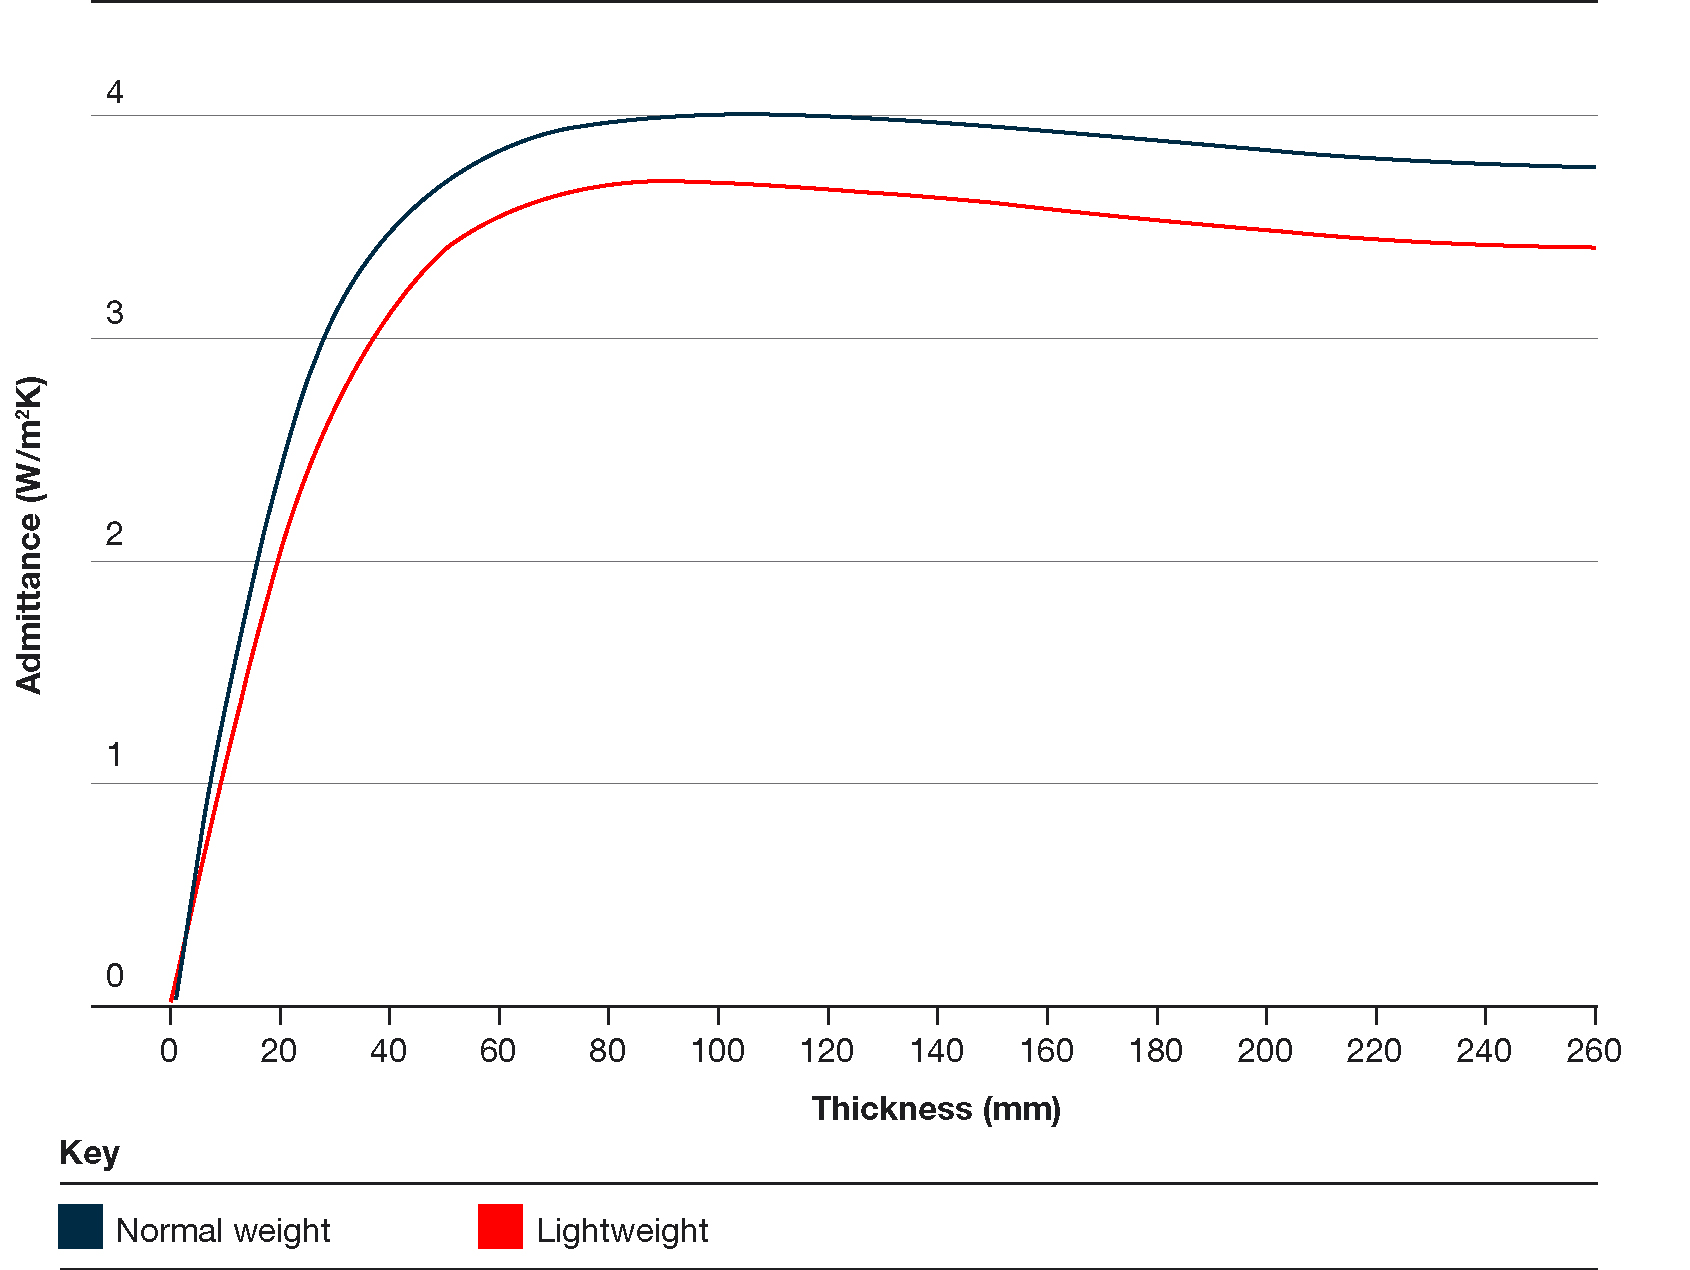
\includegraphics[scale=.7]{PIC/CH02/ADMITTANCE}
\caption{Admittance of normal and lightweight concrete remains unchanged beyond depths of \SI{100}{\mm} (\href{https://www.steelconstruction.info/File:CSD126_N7.jpg}{\url{https://www.steelconstruction.info/File:CSD126_N7.jpg}})}
\end{figure}
A typical slab in a steel building (\SIrange{75}{100}{\mm} thick) provides almost the maximum admittance (i.e., ability of the building element to store and release heat) in a naturally ventilated building as shown below. Adding concrete mass solely for passive `fabric energy storage' is therefore not effective (SSC).

Steel structures are known for:
\begin{itemize}
\item A high structural efficiency, i.e., a small amount of material provides considerable strength \& stiffness.
\item `Lean' construction, i.e., highly planned construction with little waste.
\item Flexibility and adaptability. For example, long spans mean that internal configurations may easily be changed without any major work; extensions are also relatively easy; web openings or cellular beams allow easy service integration. This extends the building life and allows greater value to be extracted from the resources invested in it.
\item Durability and Maintenance. Steel components are durable and require little maintenance in a well designed environment.
\item Recyclability. Steel is almost \si{100\percent} recyclable so it does not fill the waste dumps reducing end of life impacts. Much is currently recycled.
\end{itemize}

A 2006 BRANZ study indicated that whole of life costs for steel, timber and concrete options for two particular government buildings were within \SI{5}{\percent} of each other. The study mentions that some recycling advantages of steel and concrete buildings, which may affect the final decision about what type of building should be used, were not included.
\section{Structural Steel}
Structural steel is \textbf{an alloy of icon and carbon plus small amount of other elements, e.g., silicon (\ce{Si}), manganese (\ce{Mn}), magnesium (\ce{Mg}), copper (\ce{Cu}).} Check this video: \href{https://www.youtube.com/watch?v=PaGJwOPg2kU}{Understanding Metals}\footnote{https://www.youtube.com/watch?v=PaGJwOPg2kU}.

Common types include:
\begin{itemize}
\item \textbf{carbon steels} --- typical $f_y=\qtyrange{200}{350}{\mpa}$\\
The name comes from the reality that they contain a very small amount of other alloying elements. More carbon causes
\begin{itemize}
\item high strength
\item lower ductility
\item less weldability
\end{itemize}
\item \textbf{high strength low alloy (HSLA) steels} --- typical $f_y=\qtyrange{280}{500}{\mpa}$\\
They provide better mechanical properties or greater resistance to corrosion than carbon steels.
\item \textbf{alloy steels} --- typical $f_y=\qtyrange{550}{800}{\mpa}$\\
They are alloyed with a variety of elements in total amounts from \SIrange{1}{50}{\percent} by weight to improve its mechanical properties.
\begin{itemize}
\item heat treated (heated to \SI{900}{\celsius}) and cooled rapidly in water (quenched) to make a hard, strong and brittle structure), then it is reheated to \SI{620}{\celsius} and cooled slowly (tempered) reducing strength and increasing toughness and ductility
\item no distinct yield point, \SI{0.2}{\percent} offset strain is used
\end{itemize}
\end{itemize}
\subsection{Material Properties}
The following typical values are used for material properties of structural steel.
\begin{table}[H]
\centering
\begin{tabular}{lcc}
	\toprule
	Young's modulus (elastic modulus)                     &   $E$    &      \SI{200}{\giga\pascal}      \\
	shear modulus                                         &   $G$    &  $\approx\SI{80}{\giga\pascal}$  \\
	Poisson's ratio                                       &  $\nu$   &        $\approx\num{0.3}$        \\
	density                                               &  $\rho$  & \SI{7850}{\kilogram\per\meter^3} \\
	coefficient of thermal expansion at \SI{20}{\celsius} & $\alpha$ &    \SI{11.7E-6}{\per\celsius}    \\ \bottomrule
\end{tabular}
\end{table}
\subsection{Material Attributes}
\begin{table}[H]
\centering
\begin{tabular}{l|m{10cm}}
	\toprule
	\textbf{Attributes}                  & \textbf{Benefits}                                                                   \\ \midrule
	\textbf{High Strength}               & long spans in bridges and buildings                                                 \\ \midrule
	\textbf{Uniformity}                  & quality is generally consistent                                                     \\
	                                     & strength does not change with loading direction                                     \\ \midrule
	\textbf{Linear Elasticity}           & previous cycles of elastic loading generally make no difference to behaviour        \\
	                                     & stiffness may be calculated (e.g., $EI$, $EA$)                                      \\
	                                     & creep is not generally a problem                                                    \\
	                                     & strength does not generally change with time                                        \\ \midrule
	\textbf{Ductility}                   & can reach high strain before fracture                                               \\
	                                     & local yielding at stress concentration causes spreading of load and avoids fracture \\
	                                     & deforms slowly over time when overloaded                                            \\ \midrule
	\textbf{Toughness}                   & absorbs a large amount of energy                                                    \\ \midrule
	\textbf{Connectability}              & solid connections with welds or bolts                                               \\ \midrule
	\textbf{Prefabrication Ability}      & can be erected fast with high quality                                               \\
	                                     & good for fast--track construction, standardization                                  \\ \midrule
	\textbf{High Strength-to-Cost Ratio} & economy                                                                             \\ \midrule
	\textbf{UV Resistant}                & does not generally become brittle with time                                         \\ \midrule
	\textbf{Recyclable}                  &                                                                                     \\ \bottomrule
\end{tabular}
\end{table}
Steel, like concrete, timber and composite materials is affected by environmental factors. Unprotected steel may corrode in a hostile environment, while concrete may have `concrete cancer', timber may rot or be attacked by bugs, and composite materials may be UV sensitive. Because corrosion occurs on the surface of steel, it is often observed easily and treated. All of steel, concrete, timber and composite materials are affected by fatigue and fire too.
\subsection{Typical Mechanical Behaviour}
The typical mechnical response of structural steel shown in \figref{fig:steel_response} consists of three stages: elastic range, yield plateau and strain hardening range. Since the upper yield stress is not reliable, the lower yield stress conservatively used as the design yield stress.
\begin{figure}[H]
\centering
\footnotesize\begin{tikzpicture}
\draw[dashed](1.02,3.5)--(0,3.5)node[left]{$f_y$};
\draw[dashed](6,4.2)--(0,4.2)node[left]{$f_u$};
\draw[dashed](1,4)--(1,0)node[below]{$\varepsilon_y$};
\draw[dashed](4,3.5)--(4,0)node[below]{$\varepsilon_{sh}$};
\draw[->](-1,0)--(10,0)node[below=5mm]{strain ($\varepsilon$)};
\draw[->](0,-1)--(0,5)node[right=5mm]{stress ($f$)};
\draw[very thick,line join=round](0,0)--(1,4)node[red,thick,circle,draw,inner sep=0,minimum size=2mm]{}node[above=1mm,anchor=south west,fill=white]{upper yield stress}--(1.02,3.5);
\draw[very thick,line join=round,decoration={random steps,segment length=2.5pt,amplitude=1pt}]decorate{(1.02,3.5)--(4,3.5)node[below=4mm,midway,fill=white]{lower yield stress}};
\draw[very thick](4,3.5)to[out=30,in=180](6,4.2)node[red,thick,circle,draw,inner sep=0,minimum size=2mm]{}to[out=0,in=160](8,3.8)node[red]{\Huge\texttimes}node[right=5mm]{tension};
\node at(8,3.5){fracture};
\draw[very thick,dashed](4,3.5)to[out=40,in=185](9,5)node[right=5mm]{compression};
\draw[very thick,dashed](4,3.5)to[out=35,in=180](8,4.4)node[right=5mm]{true};
\draw[|-|](0,-.6)--++(1,0)node[midway,below=2mm,anchor=north,fill=white]{elastic range};
\draw[|-|](1,-.6)--++(3,0)node[midway,below=2mm,anchor=north,fill=white]{yield plateau};
\draw[|->](4,-.6)--++(4,0)node[midway,below=2mm,anchor=north,fill=white]{strain hardening range};
\node at(8,1.5){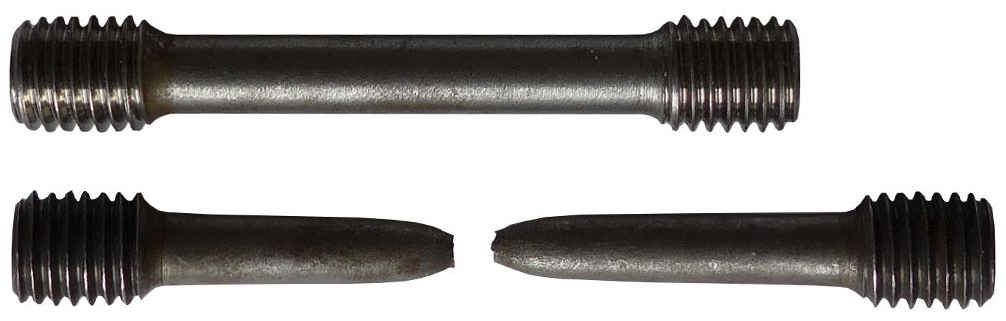
\includegraphics[width=7cm]{PIC/CH02/DT}};
\draw[line width=1mm,cc0066,->](4.2,2.1)--++(-1,0);
\draw[line width=1mm,cc0066,->](10.4,2.1)--++(1,0);
\end{tikzpicture}

\caption{Typical strain--stress response of steel}\label{fig:steel_response}
\end{figure}
Depending on different strain/stress measures, the response may be different. Sometimes engineers use true strain and true stress (instead of engineering strain and stress) to characterise material response. The difference could be significant when deformation is large, interested readers can check this video: \href{https://www.youtube.com/watch?v=AkX6JqlWRqc}{Understanding True Stress and True Strain}\footnote{https://www.youtube.com/watch?v=AkX6JqlWRqc}.
\begin{figure}[H]
\centering
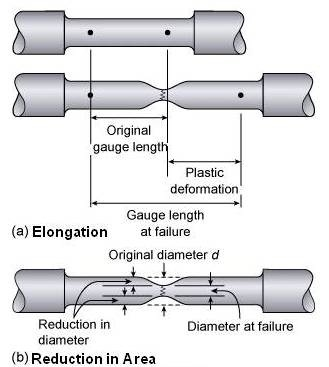
\includegraphics[scale=.8]{PIC/CH02/TA}
\caption{Nominal and true area}
\end{figure}

For idealised response, often the upper yield stress is ignored, resulting in the following idealised curves as shown in \figref{fig:steel_responses}. For alloy steel, since there is no explicit yielding point, often it is set to the stress corresponds to \SI{0.2}{\percent} offset strain.
\begin{figure}[H]
\centering
\footnotesize\begin{tikzpicture}
\newdimen\XCoord
\newdimen\YCoord
\newcommand*{\ExtractCoordinate}[1]{\path (#1); \pgfgetlastxy{\XCoord}{\YCoord};}
\draw[->](0,0)--(10,0)node[below=3mm]{tension strain ($\varepsilon$)};
\draw[->](0,0)--(0,6)node[left=5mm]{stress ($f$)};
\draw[very thick,line join=round](0,0)--(.5,2)--(3,2)to[out=30,in=180](6,2.8)to[out=0,in=160](8,2.4)node[right=5mm]{low carbon steel};
\draw[very thick,line join=round](0,0)--(.8,3.2)--(3,3.2)to[out=30,in=180](6,3.8)to[out=0,in=160](8,3.4)node[right=5mm]{HSLA steel};
\draw[very thick,line join=round,name path=s](0,0)--(1,4)to[out=76,in=210](3,5)to[out=30,in=180](5,5.5)to[out=0,in=110](7,4)node[right=5mm]{alloy steel};
\draw[dashed,name path=e](.1,0)--++(1.25,5)node[above]{\SI{0.2}{\percent} offset};
\path[name intersections={of=s and e,by=sy}];
\ExtractCoordinate{$(sy)$}
\draw(sy)node[fill=red,inner sep=0,minimum size=2mm,circle]{}node[align=left,below right=1mm,fill=white,anchor=north west]{yield stress\\for alloy steel};
\draw[dashed](sy)--(\XCoord,0);
\draw[|<->|](0,-.4)--++(\XCoord,0)node[midway,fill=white]{\SI{0.5}{\percent}};
\draw[dashed](sy)--(0,\YCoord)node[left=2mm]{$\approx\SI{700}{\mpa}$};
\draw[dashed](3,3.2)--(0,3.2)node[left=2mm]{$\approx\SI{350}{\mpa}$};
\draw[dashed](3,2)--(0,2)node[left=2mm]{$\approx\SI{250}{\mpa}$};
\node at(7,1){(not to scale)};
\end{tikzpicture}

\caption{Idealised strain--stress responses of various types of steel}\label{fig:steel_responses}
\end{figure}
\subsection{Common Grades}
The most common type of Australasian structural steel grades for hot--rolled structural steel bars and sections (including universal sections, taper flange beams, angles and channels) are given below. All of these grades are weldable and come with subgrades of L0 and L15 indicating low (\SI{27}{\joule} at \SI{0}{\celsius}) and high (\SI{27}{\joule} at \SI{-15}{\celsius}) \href{https://www.youtube.com/watch?v=tpGhqQvftAo}{Charpy V-notch}\footnote{https://www.youtube.com/watch?v=tpGhqQvftAo} toughnesses respectively. For a UB or UC section, coupons to determine the yield stress of a section are to be taken from the flange.
\begin{table}[H]
\centering\footnotesize\caption{Tensile test requirements for flats and sections}\label{tab:ys}
\begin{tabular}{l|cccc|c|c}
	\toprule
	\multirow{3}[0]{*}{\centering{}grade} &        \multicolumn{4}{c|}{minimum yield stress $f_y$ (\si{\mpa})}        & \multicolumn{1}{c|}{\multirow{2}[0]{*}{\parbox{2.5cm}{\centering{}minimum tensile strength $f_u$}}} & \multicolumn{1}{c}{\multirow{2}[0]{*}{\parbox{2cm}{\centering{}minimum elongation}}} \\
	                                      &                 \multicolumn{4}{c|}{thickness (\si{\mm})}                 &                                                                                                     &                                                                                      \\
	                                      & $<11$ & $\geqslant11$ and $\leqslant17$ & $>17$ and $<40$ & $\geqslant40$ &                                              \si{\mpa}                                              &                                    \si{\percent}                                     \\ \midrule
	300, 300L0                            &  320  &               300               &       280       &      280      &                                                 440                                                 &                                          22                                          \\
	300L15, 300S0                         &  320  &               300               &       280       &      280      &                                                 440                                                 &                                          25                                          \\
	350, 350L0                            &  360  &               340               &       340       &      330      &                                                 480                                                 &                                          20                                          \\
	350S0, 350L15                         &  360  &               340               &       340       &      330      &                                                 480                                                 &                                          25                                          \\ \bottomrule
	\multicolumn{7}{l}{Please refer to \ASNZSSTEEL{Table 14} for notes and details.}
\end{tabular}
\end{table}
\begin{table}[H]
\centering\footnotesize
\caption{Tensile test requirements for cold--formed hollow sections}
\begin{tabular}{l|cc}
	\toprule
	\multirow{2}[0]{*}{grade} & minimum yield stress $f_y$ & minimum tensile strength $f_u$ \\
	                          &     \si{\mpa}      &       \si{\mpa}        \\ \midrule
	C250, C250L0              &            250             &              320               \\
	C350, C350L0              &            350             &              430               \\
	C450, C450L0              &            450             &              500               \\ \bottomrule
	\multicolumn{3}{l}{Please refer to \ASNZSCOLD{Table 7} for notes and details.}
\end{tabular}
\end{table}
\begin{table}[H]
\centering\footnotesize
\caption{Tensile test requirements for plate and floor plate}\label{tab:plate}
\begin{tabular}{c|cccccccc|ccc}
	\toprule
	\multirow{3}[0]{*}{grade} &                                         \multicolumn{8}{c|}{minimum $f_y$ (\si{\mpa})}                                         &  \multicolumn{3}{c}{minimum $f_u$ (\si{\mpa})}  \\
	                          &                                         \multicolumn{8}{c|}{thickness $t$ (\si{\mm})}                                          &  \multicolumn{3}{c}{thickness $t$ (\si{\mm})}   \\
	                          &              &     $>8$      &     $>12$     &     $>20$     &     $>32$     &     $>50$     &     $>80$      &     $>150$     &               &     $>20$      &     $>150$     \\
	                          & $\leqslant8$ & $\leqslant12$ & $\leqslant20$ & $\leqslant32$ & $\leqslant50$ & $\leqslant80$ & $\leqslant150$ & $\leqslant200$ & $\leqslant20$ & $\leqslant150$ & $\leqslant200$ \\ \midrule
	           200            &     200      &      200      &               &               &               &               &                &                &      300      &      300       &      290       \\
	           250            &     280      &      260      &      250      &      250      &      250      &      240      &      230       &      220       &      410      &      410       &      400       \\
	           300            &     320      &      310      &      300      &      280      &      280      &      270      &      260       &      250       &      430      &      430       &      420       \\
	           350            &     360      &      360      &      350      &      340      &      340      &      340      &      330       &      320       &      450      &      450       &      450       \\
	           400            &     400      &      400      &      380      &      360      &      360      &      360      &                &                &      480      &      480       &                \\
	           450            &     450      &      450      &      450      &      420      &      400      &               &                &                &      520      &      500       &                \\
	          WR350           &     340      &      340      &      340      &      340      &      340      &      340      &                &                &      450      &      450       &                \\ \bottomrule
	\multicolumn{12}{l}{Please refer to \ASNZSPLATE{Table 8} for notes and details.}
\end{tabular}
\end{table}
\section{Design Yield Stress for Sections}\label{sec:ys}
For members of uniform thickness (such as plates, angles, etc.), the yield stress may be obtained directly for the appropriate material grade. However, a number of different member types do not have uniform thickness. This includes I-sections, C-sections, etc., where the thickness of flanges is generally greater than that of webs. While the different strengths of the different components (e.g., webs, flanges.) could be used in the calculations, this is usually too cumbersome for routine design, and the increase in accuracy is generally small. It is therefore reasonable to use the following rules:
\begin{itemize}
\item For bending (flexural) strength (about both strong and weak axes, see sketches below), use \boldmath{$f_y=f_{y,flange}$} as flanges are the main contributors to resistance.
\begin{figure}[H]
\centering
\begin{tikzpicture}
\draw[dashed](-5,0)--(3,0);
\draw[dashed](2,-1.5)--++(0,3);
\draw[fill=black!20](2,-1)|-++(1,2)--++(-2,-2)--cycle;
\draw[line width=2mm,black!40](-2,0)--++(2,0);
\draw[line width=2mm,cc0066](-2,-1)--++(0,2)(0,-1)--++(0,2);
\draw[line width=2mm,black!40](-4,-1)--++(0,2);
\draw[line width=2mm,cc0066](-5,-1)--++(2,0)(-5,1)--++(2,0);
\end{tikzpicture}
\end{figure}
\item For axial strength, use \boldmath{$f_y=f_{y,flange}$} as both web and flanges contribute to resistance but $f_{y,flange}$ is often smaller, which leads to conservative design.
\begin{figure}[H]
\centering
\begin{tikzpicture}
\draw[dashed](-2,0)--(3,0);
\draw[dashed](2,-1.5)--++(0,3);
\draw[fill=black!20](2,-1)rectangle++(1,2);
\draw[line width=2mm,cc0066](-1,-1)--++(0,2);
\draw[line width=2mm,cc0066](-2,-1)--++(2,0)(-2,1)--++(2,0);
\end{tikzpicture}
\end{figure}
\item For shear strength associated with strong--axis bending, use \boldmath{$f_y=f_{y,web}$} as web is the main contributor to resistance.
\begin{figure}[H]
\centering
\begin{tikzpicture}
\draw[dashed](-2,0)--(3,0);
\draw[dashed](2,-1.5)--++(0,3);
\draw[fill=black!20](2,-1.05)--(2.1,-.95)--(2.5,-.95)to[out=0,in=-90](3,0)to[out=90,in=0](2.5,.95)--(2.1,.95)--(2,1.05)--cycle;
\draw[line width=2mm,black!40](-2,-1)--++(2,0)(-2,1)--++(2,0);
\draw[line width=2mm,cc0066](-1,-1.1)--++(0,2.2);
\end{tikzpicture}
\end{figure}
\item For shear strength associated with weak--axis bending, use \boldmath{$f_y=f_{y,flange}$} as flanges are the main contributors to resistance.
\begin{figure}[H]
\centering
\begin{tikzpicture}
\draw[dashed](-2,0)--(3,0);
\draw[dashed](2,-1.5)--++(0,3);
\draw[fill=black!20](2,-1)to[out=20,in=-90](3,0)to[out=90,in=-20](2,1)--cycle;
\draw[line width=2mm,black!40](-2,0)--++(2,0);
\draw[line width=2mm,cc0066](-2,-1)--++(0,2)(0,-1)--++(0,2);
\end{tikzpicture}
\end{figure}
\end{itemize}
\section{Structural Shapes}
Common types include:
\begin{itemize}
\item hot--formed\\Steel is formed into the shape of the section while it is still hot. Many kinds of working, including rolling, forging, extrusion and drawing, can be done with hot metal.
\item cold--formed\\Thin plate steel is shaped by cold--working processes carried out near room temperature, such as rolling, pressing, stamping, bending, etc.
\item built--up\\Steel is formed by welding together plates to form various section shapes.
\end{itemize}
We will not use cold--formed sections in this course. For availability, readers can refer to specification manual provided by Liberty Steel.
\subsection{Hot--Rolled Products}
\begin{enumerate}[itemsep=1em]
\item Universal Beams (UB)\qquad\ASNZSSTEEL{~}\\[1em]
\begin{minipage}[t]{9cm}
Different names may be used in other codes. For example, I-Beam --- NZ/AU/UK; H-Section --- Japan; WF-Beam --- USA; IPE, HE, HL, HD --- EU. A typical designation consists of three components.
\begin{table}[H]\centering
\begin{tabular}{ccc}
	  \textbf{460}   & \textbf{UB} &       \textbf{74.6}        \\
	\textbf{approx.} &  universal  &           linear           \\
	     depth       &    beam     &          density           \\
	   (\si{\mm})    &             & (\si{\kilogram\per\meter})
\end{tabular}
\end{table}
Linear density is the mass per unit length. The depth is greater than the flange width.
\begin{itemize}
\item high flexural strength to area ratio
\item high flexural stiffness to area ratio
\item high moment capacity due to high lever arm
\item flanges and webs are easy to bolt (flat)
\item thickness of flange/web selected to limit buckling
\end{itemize}
\end{minipage}\hfill
\begin{minipage}[t]{5cm}
\centering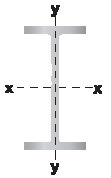
\includegraphics[width=4.5cm,valign=t]{PIC/CH02/UB}
\end{minipage}
\item Universal Columns (UC)\qquad\ASNZSSTEEL{~}\\[1em]
\begin{minipage}[t]{9cm}
Similar to UB, a typical designation consists of three components.
\begin{table}[H]\centering
\begin{tabular}{ccc}
	\textbf{250} & \textbf{UC} &       \textbf{72.9}        \\
	  approx.    &  universal  &           linear           \\
	   depth     &   column    &          density           \\
	 (\si{\mm})  &             & (\si{\kilogram\per\meter})
\end{tabular}
\end{table}
The geometry of UC sections differ from UB sections with wider flanges in order to limit lateral buckling. The depth is similar to the flange width.

The radius of gyration $r_y=\sqrt{\dfrac{I_{y}}{A}}$ about weak axis is often larger than that of UB sections.
\end{minipage}\hfill
\begin{minipage}[t]{5cm}
\centering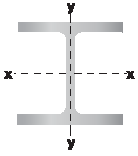
\includegraphics[width=4.5cm,valign=t]{PIC/CH02/UC}
\end{minipage}
\item Universal Bearing Piles (UBP), a.k.a., H sections\\[1em]
\begin{minipage}[t]{9cm}
A typical designation:
\begin{table}[H]\centering
\begin{tabular}{ccc}
	\textbf{310} & \textbf{UBP}  &        \textbf{149}        \\
	  approx.    &   universal   &           linear           \\
	   depth     & bearing piles &          density           \\
	 (\si{\mm})  &               & (\si{\kilogram\per\meter})
\end{tabular}
\end{table}
UBP sections are similar to UC sections but have uniform thickness for both web and flanges.
\end{minipage}\hfill
\begin{minipage}[t]{5cm}
\centering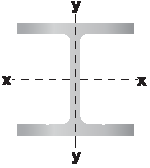
\includegraphics[width=4.5cm,valign=t]{PIC/CH02/UBP}
\end{minipage}
\item Parallel Flange Channels (PFC)\\[1em]
\begin{minipage}[t]{9cm}
A typical designation:
\begin{table}[H]\centering
\begin{tabular}{cc}
	\textbf{200} &  \textbf{PFC}  \\
	  section    &    parallel    \\
	   depth     & flange channel \\
	 (\si{\mm})  &
\end{tabular}
\end{table}
\end{minipage}\hfill
\begin{minipage}[t]{5cm}
\centering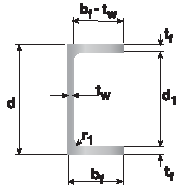
\includegraphics[width=4.5cm,valign=t]{PIC/CH02/PFC}
\end{minipage}
\item Tapered Flange Beams (TFB)\\[1em]
\begin{minipage}[t]{9cm}
Sometimes TFB is also called Rolled Steel Joinst (RSJ), M, S sections. A typical designation:
\begin{table}[H]\centering
\begin{tabular}{cc}
	\textbf{125} & \textbf{TFB} \\
	  section    &   tapered    \\
	   depth     & flange beam  \\
	 (\si{\mm})  &
\end{tabular}
\end{table}
TFBs are traditional sections. However, there are deemed as inefficient structural member. Sloping washers are needed for flange connections.
\end{minipage}\hfill
\begin{minipage}[t]{5cm}
\centering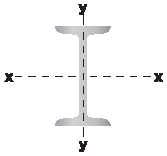
\includegraphics[width=4.5cm,valign=t]{PIC/CH02/TFB}
\end{minipage}
\item Taper Flange Channels (TFC)\\[1em]
\begin{minipage}[t]{9cm}
Traditionally often used for framing around door opening, or for built-up lattices members. Seldom used now.
\end{minipage}\hfill
\begin{minipage}[t]{5cm}
\centering\begin{tikzpicture}[baseline=(A.base)]
\node(A)at(0,3){};
\draw[pattern=north west lines](0,0)--(2,0)arc(0:90:.2)--(.2,.4)--(.2,2.6)--(1.8,2.8)arc(-90:0:.2)--(0,3)--cycle;
\end{tikzpicture}
\end{minipage}
\item Equal Angles (EA)\\[1em]
\begin{minipage}[t]{9cm}
Angles are commonly used as tension bracing or for built--up members.

A typical designation:
\begin{table}[H]\centering
\begin{tabular}{cccccc}
	 \textbf{125}  & \textbf{\texttimes} &  \textbf{125}  & \textbf{\texttimes} &  \textbf{16}   & \textbf{EA} \\
	$a$ (\si{\mm}) &                     & $b$ (\si{\mm}) &                     & $t$ (\si{\mm}) &
\end{tabular}
\end{table}

It is also denoted as L125\texttimes125\texttimes16 or 125\texttimes16EA.
\end{minipage}\hfill
\begin{minipage}[t]{5cm}
\centering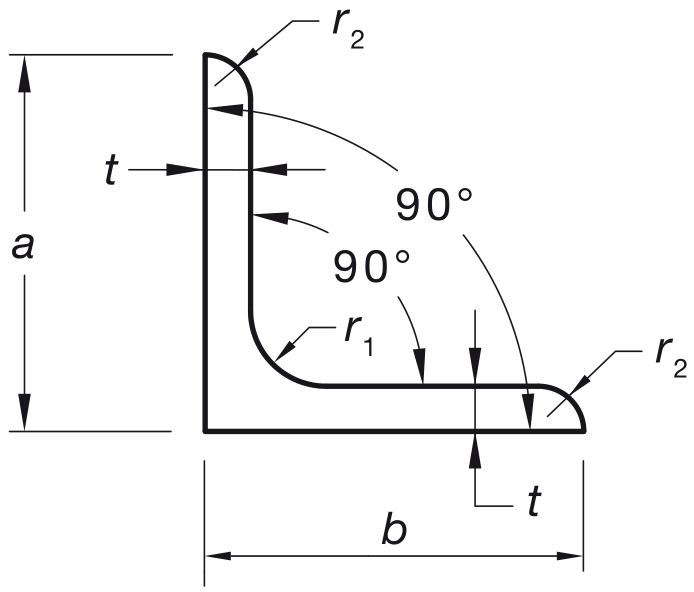
\includegraphics[width=4.5cm,valign=t]{PIC/CH02/EA}
\end{minipage}
\item Unequal Angles (UA)\\[1em]
\begin{minipage}[t]{9cm}
Angles are commonly used as tension bracing or for built--up members.

A typical designation:
\begin{table}[H]\centering
\begin{tabular}{cccccc}
	 \textbf{125}  & \textbf{\texttimes} &  \textbf{75}   & \textbf{\texttimes} &  \textbf{12}   & \textbf{UA} \\
	$a$ (\si{\mm}) &                     & $b$ (\si{\mm}) &                     & $t$ (\si{\mm}) &
\end{tabular}
\end{table}
It is also denoted as L125\texttimes75\texttimes12UA.
\end{minipage}\hfill
\begin{minipage}[t]{5cm}
\centering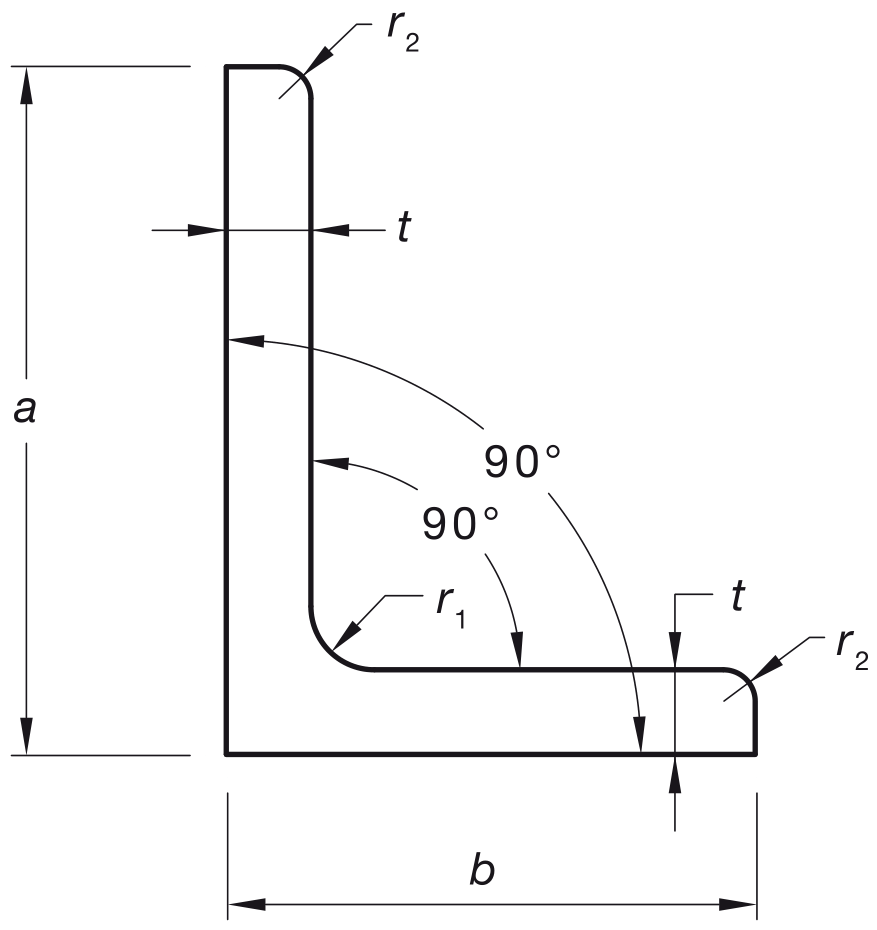
\includegraphics[width=4.5cm,valign=t]{PIC/CH02/UA}
\end{minipage}
\item Structural Tees (T)\\[1em]
\begin{minipage}[t]{9cm}
They can be made by splitting UC or UB sections and used for chord members in steel trusses, flanges in plate girders or hangers.
\end{minipage}\hfill
\begin{minipage}[t]{5cm}
\centering\begin{tikzpicture}[x=1cm,y=1cm,scale=.5,baseline=(A.base)]
\node(A)at(0,3){};
\draw[pattern=north west lines](-.25,0)rectangle(.25,3);
\draw[pattern=north west lines](-2.5,3)rectangle(2.5,3.5);
\draw[dashed](-.25,-3)rectangle(.25,3);
\draw[dashed](-2.5,-3.5)rectangle(2.5,-3);
\end{tikzpicture}
\end{minipage}
\item Rectangular Hollow Sections (RHS)\\[1em]
\begin{minipage}[t]{9cm}
A typical designation:
\begin{table}[H]\centering
\begin{tabular}{cccccc}
	 \textbf{75}   & \textbf{\texttimes} &  \textbf{25}   & \textbf{\texttimes} &  \textbf{2.5}  & \textbf{RHS} \\
	$d$ (\si{\mm}) &                     & $b$ (\si{\mm}) &                     & $t$ (\si{\mm}) &
\end{tabular}
\end{table}
\end{minipage}\hfill
\begin{minipage}[t]{5cm}
\centering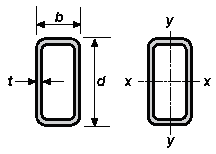
\includegraphics[width=4.5cm,valign=t]{PIC/CH02/RHS}
\end{minipage}
\item Circular Hollow Sections (CHS)\\[1em]
\begin{minipage}[t]{9cm}
A typical designation:
\begin{table}[H]\centering
\begin{tabular}{cccc}
	 \textbf{165.1}  & \textbf{\texttimes} &  \textbf{3.0}  & \textbf{CHS} \\
	$d_0$ (\si{\mm}) &                     & $t$ (\si{\mm}) &
\end{tabular}
\end{table}
\end{minipage}\hfill
\begin{minipage}[t]{5cm}
\centering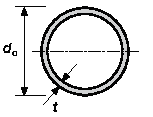
\includegraphics[width=4.5cm,valign=t]{PIC/CH02/CHS}
\end{minipage}
\item Plates

Common thicknesses include: \SI{5}{\mm}, \SI{6}{\mm}, \SI{8}{\mm}, \SI{10}{\mm}, \SI{12}{\mm}, \SI{16}{\mm}, \SI{20}{\mm}, \SI{25}{\mm}. Common widths include: \SI{20}{\mm}, \SI{25}{\mm}, \SI{32}{\mm}, \SI{40}{\mm}, \SI{50}{\mm}, \SI{65}{\mm}, \SI{75}{\mm}, \SI{90}{\mm}, \SI{100}{\mm}, \SI{110}{\mm}, \SI{130}{\mm}, \SI{150}{\mm}.

e.g., 12\texttimes200\texttimes300 plate.
\item Bars

Flat bars, commonly also referred to as `flats', commonly have widths ranging from \SI{10}{\mm} to \SI{90}{\mm}.

e.g., 12\texttimes24\texttimes300 bar.
\end{enumerate}

Sections may also be described in terms of being non-symmetric, singly symmetric or doubly symmetric. For example,
\begin{figure}[H]
\centering
\footnotesize
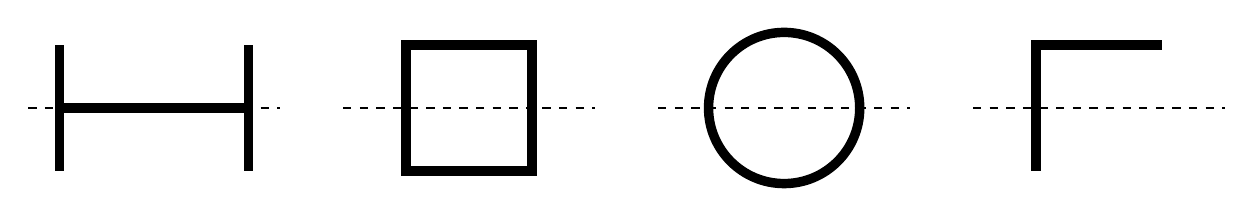
\begin{tikzpicture}[scale=.8]
\begin{scope}
\draw[line width=1.2mm](-1.5,-1)--++(0,2)(1.5,-1)--++(0,2)(-1.5,0)--++(3,0);
\draw[dashed](-2,0)--++(4,0);
\end{scope}
\begin{scope}[xshift=5cm]
\draw[line width=1.2mm](-1,-1)rectangle(1,1);
\draw[dashed](-2,0)--++(4,0);
\end{scope}
\begin{scope}[xshift=10cm]
\draw[line width=1.2mm](0,0)circle(1.2cm);
\draw[dashed](-2,0)--++(4,0);
\end{scope}
\begin{scope}[xshift=15cm]
\draw[line width=1.2mm](-1,-1)|-(1,1);
\draw[dashed](-2,0)--++(4,0);
\end{scope}
\end{tikzpicture}
\caption{Examples of non-symmetric, singly symmetric and doubly symmetric sections}
\end{figure}
\subsection{Cold--Formed Products}
\begin{figure}[H]
\centering
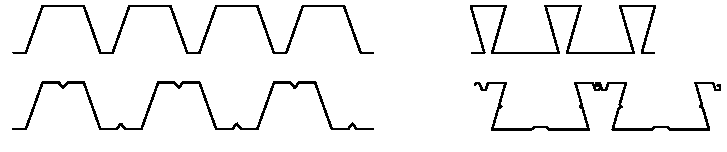
\includegraphics[width=.9\textwidth]{PIC/CH02/SHEET}
\caption{Profiled sheets and linear trays \citep{Dubina2012}}
\end{figure}
\begin{figure}[H]
\centering
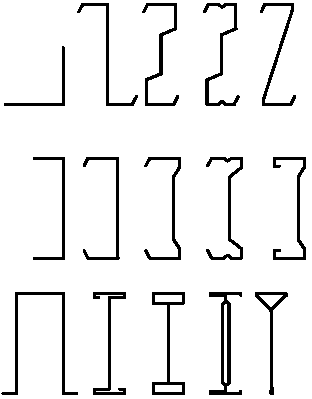
\includegraphics[width=.45\textwidth]{PIC/CH02/OPEN}
\caption{Single open sections \citep{Dubina2012}}
\end{figure}
\begin{figure}[H]
\centering
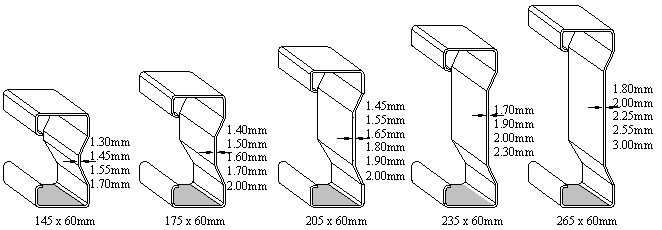
\includegraphics[width=.9\textwidth]{PIC/CH02/SUM}
\caption{Channel sections \citep{Dubina2012}}
\end{figure}
\subsection{Standard Welded Products}
Welded sections are often welded together plates. They can be welded on either one side only or both sides.

\begin{minipage}[t]{9cm}
\begin{enumerate}
\item Welded Beams (WB)\\
A typical designation:
\begin{table}[H]\centering
\begin{tabular}{ccc}
	\textbf{900} & \textbf{WB} &        \textbf{218}        \\
	    $d$      &   welded    &           linear           \\
	   height    &    beam     &          density           \\
	 (\si{\mm})  &             & (\si{\kilogram\per\meter})
\end{tabular}
\end{table}
\item Welded Columns (WC)\\
A typical designation:
\begin{table}[H]\centering
\begin{tabular}{ccc}
	\textbf{400} & \textbf{WC} &        \textbf{270}        \\
	    $d$      &   welded    &           linear           \\
	   height    &   column    &          density           \\
	 (\si{\mm})  &             & (\si{\kilogram\per\meter})
\end{tabular}
\end{table}
\end{enumerate}
\end{minipage}\hfill
\begin{minipage}[t]{5cm}
\vfill\centering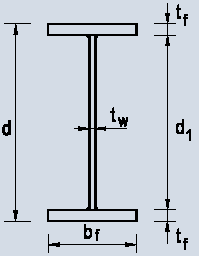
\includegraphics[width=4.5cm,valign=t]{PIC/CH02/WB}
\end{minipage}

Non-prismatic sections can be used to reduce cost and improve efficiency, e.g.,
\begin{figure}[H]
\centering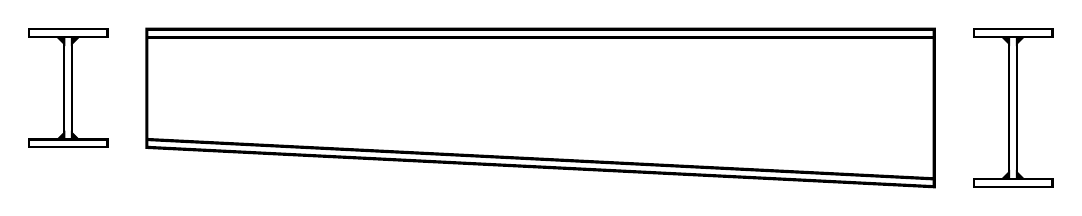
\begin{tikzpicture}
\begin{scope}[line width=.4mm]
\draw(0,-.5)--++(0,1.5)--++(10,0)--++(0,-2)--cycle;
\draw(0,.9)--(10,.9);
\draw(0,-.4)--(10,-.9);
\end{scope}
\begin{scope}[xshift=-1cm,thick]
\def\b{.1}
\draw(-.5,-.5)rectangle++(1,\b);
\draw(-.5,1)rectangle++(1,-\b);
\draw(-.5*\b,-.5+\b)rectangle++(\b,1.5-2*\b);
\def\a{.08}
\draw[fill](-.05-\a,-.5+\b)--++(\a,\a)|-cycle;
\draw[fill](.05+\a,-.5+\b)--++(-\a,\a)|-cycle;
\draw[fill](-.05-\a,1-\b)--++(\a,-\a)|-cycle;
\draw[fill](.05+\a,1-\b)--++(-\a,-\a)|-cycle;
\end{scope}
\begin{scope}[xshift=11cm,thick]
\def\b{.1}
\draw(-.5,-1)rectangle++(1,\b);
\draw(-.5,1)rectangle++(1,-\b);
\draw(-.5*\b,-1+\b)rectangle++(\b,2-2*\b);
\def\a{.08}
\draw[fill](-.05-\a,-1+\b)--++(\a,\a)|-cycle;
\draw[fill](.05+\a,-1+\b)--++(-\a,\a)|-cycle;
\draw[fill](-.05-\a,1-\b)--++(\a,-\a)|-cycle;
\draw[fill](.05+\a,1-\b)--++(-\a,-\a)|-cycle;
\end{scope}
\end{tikzpicture}
\caption{Non-prismatic sections by plates welded together}
\end{figure}
\section{Steel Availability}
Some general guidance is available from mills which may be relevant to Australasia (e.g., Liberty Steel Hot Rolled and Structural Steel Product).

SCNZ recommends chartered distributor for sources compliant structural steel. Distributors have limited members so it is best to call the check availability.
\section{Standard Tolerance}
Sections, as well as members, must satisfy code dimension requirements (\NZSSTEEL{\S~14.4}). Deformations must arise as parts of members cool at different rates and residual stresses are developed.
\begin{figure}[H]
\centering
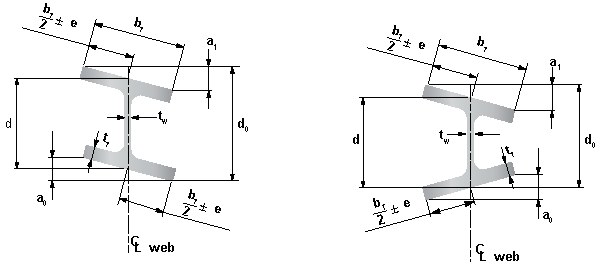
\includegraphics[width=14cm]{PIC/CH02/TOLERANCE}
\caption{Tolerances on a cross section}
\end{figure}

Typical tolerance for camber and sweep is $L/1000$ (\NZSSTEEL{Table 14.4.5}). For I sections with a flange width less than \SI{150}{\mm}, the tolerance of sweep can be as large as $L/500$.
\begin{figure}[H]
\centering
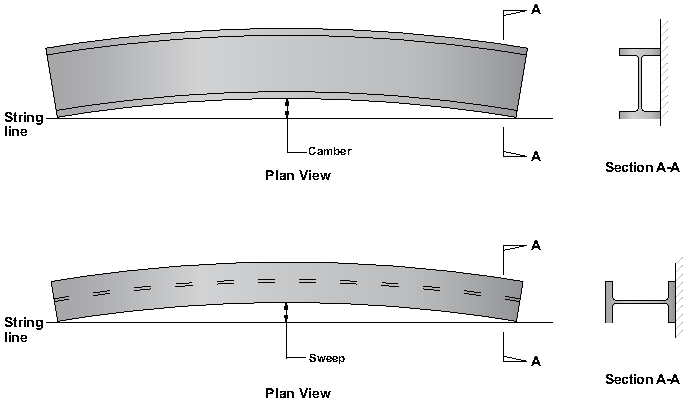
\includegraphics[width=14cm]{PIC/CH02/CAMBER}
\caption{Measurement of camber and sweep}
\end{figure}
\section{Undesirable Steel Behaviour}
\subsection{Brittle Fracture}
Brittle fracture affects strength.
\begin{figure}[H]
\centering
\begin{tikzpicture}
\draw[->](0,0)--(10,0)node[below=3mm]{strain ($\varepsilon$)};
\draw[->](0,0)--(0,6)node[left=3mm]{stress ($f$)};
\draw[very thick,line join=round](0,0)--(.5,2)--(3,2)to[out=30,in=180](6,2.8)to[out=0,in=160](8,2.4)node[red]{\LARGE\texttimes}node[right=5mm]{low carbon steel};
\draw[very thick](0,0)--(.6,2.4)node[red]{\LARGE\texttimes}node[above=2mm,fill=white]{brittle fracture};
\node at(7,4.5){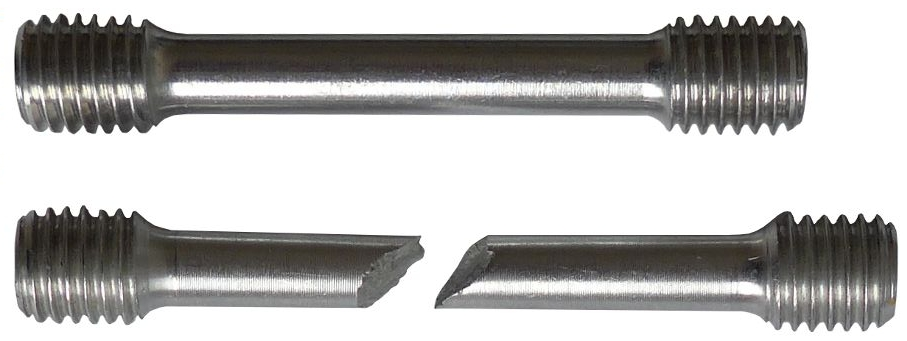
\includegraphics[width=7cm]{PIC/CH02/BRI}};
\end{tikzpicture}
\caption{Brittle fracture}
\end{figure}
\subsection{Buckling}
Structural members may fail under buckling, the material strength is not fully utilised under buckling. To learn more, check this video: \href{https://www.youtube.com/watch?v=21G7LA2DcGQ}{Understanding Buckling}\footnote{https://www.youtube.com/watch?v=21G7LA2DcGQ}.
\begin{figure}[H]
\centering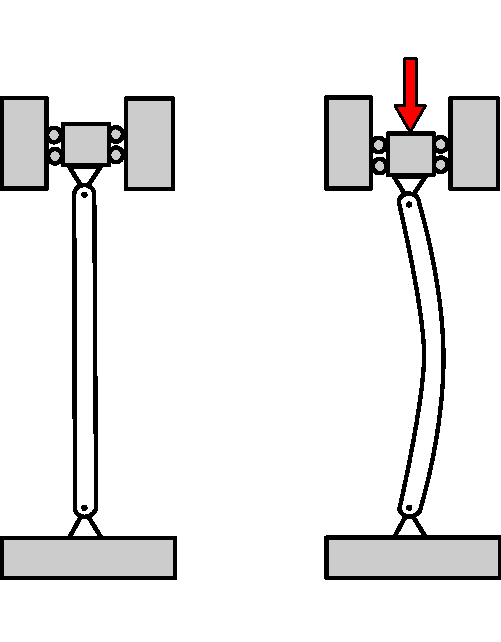
\includegraphics[height=9cm]{PIC/CH04/BUCKLING}
\caption{Buckling}
\end{figure}
\subsection{Excessive Deformation/Vibration}
It affects serviceability.
\begin{itemize}
\item bouncy floor
\item ponding
\begin{figure}[H]
\centering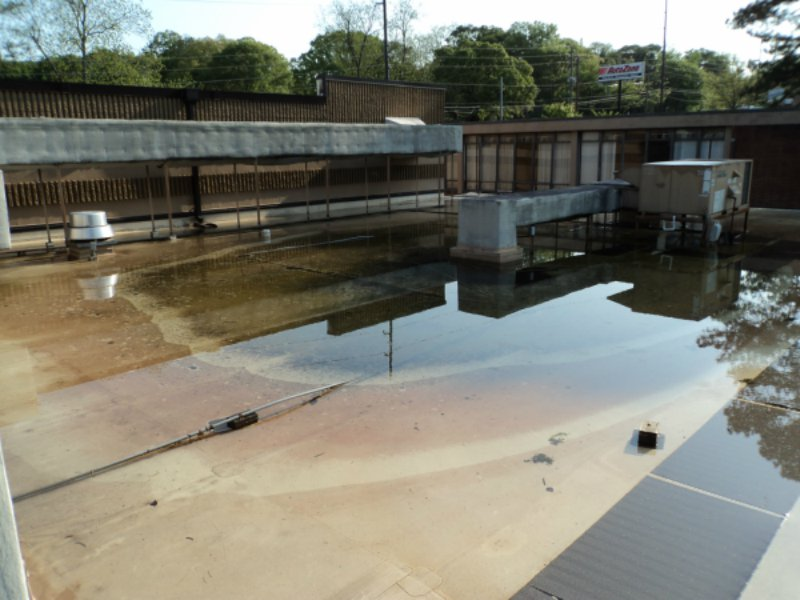
\includegraphics[height=8cm]{PIC/CH02/PONDING}
\caption{Ponding on roof}
\end{figure}
\end{itemize}
\section{Standard Gauge}
The following tables are generated according to tables from Table 10.2-1 to Table 10.2-5 provided by ASI design capacity tables \citep{ASI2016}. Please refer to ASI manual for notes.
\begin{table}[H]
\centering\footnotesize
\caption{Gauge lines for universal sections}\label{tab:universal_gauge}
\begin{minipage}{.8\linewidth}\centering
\begin{tabular}{l|rr|rr|rrr|rrr}
	\toprule
	\multirow{2}[0]{*}{Section} &        \multicolumn{4}{c|}{Flange $s_{gf}$}         &          \multicolumn{6}{c}{Web $s_{gw}$}          \\
	                            & \multicolumn{2}{c|}{M20} & \multicolumn{2}{c|}{M24} & \multicolumn{3}{c|}{M20} & \multicolumn{3}{c}{M24} \\ \midrule
	610UB                       &  140 &                90 & 140 &                 90 & 140 & 90 &            70 & 140 & 90 &           70 \\
	530UB                       &  140 &                90 & 140 &                 90 & 140 & 90 &            70 & 140 & 90 &           70 \\
	460UB                       &   90 &               140 &  90 &                    &  90 & 70 &           140 &  90 & 70 &          140 \\
	410UB                       &   90 &                70 &  90 &                    &  90 & 70 &           140 &  90 & 70 &          140 \\
	360UB,310UB                 &   90 &                70 &  90 &                    &  90 & 70 &           140 &  90 & 70 &          140 \\
	310UB32.0                   &   70 &                   &   b &                    &  90 & 70 &           140 &  90 & 70 &          140 \\
	250UB                       &   70 &                90 &   b &                    &  70 & 90 &           140 &  70 & 90 &              \\
	250UB25.7                   &  70* &                   &   b &                    &  70 & 90 &               &  70 & 90 &              \\
	200UB                       &   70 &                   &   b &                    &  70 & 90 &               &  70 & 90 &              \\
	200UB18.2                   &  60* &                   &   b &                    &  70 & 90 &               &  70 &    &              \\
	180UB                       & 50** &                   &   b &                    &  70 &    &               &  70 &    &              \\
	150UB                       &    c &                   &   b &                    &  60* &    &               &   b &    &              \\
	310UC                       &  140 &                90 & 140 &                 90 &  90 & 70 &           140 &  90 & 70 &          140 \\
	250UC                       &  140 &                90 & 140 &                 90 &  90 & 70 &           140 &  90 & 70 &              \\
	200UC                       &  140 &                90 & 140 &                 90 &  90 & 70 &               &  90 & 70 &              \\
	150UC                       &   90 &                70 &  90 &                    &  60* &    &               &   b &    &              \\
	100UC                       &  60* &                   &   b &                    &   c &    &               &   b &    &              \\
	Preference                  &    1 &                 2 &   1 &                  2 &   1 &  2 &             3 &   1 &  2 &            3 \\ \bottomrule
\multicolumn{11}{l}{* Gauge listed are for M16 bolts.}\\
\multicolumn{11}{l}{** Gauge listed are for M12 bolts.}\\
\multicolumn{11}{l}{b indicates that the flange or web cannot accommodate this size of bolt.}\\
\multicolumn{11}{l}{c indicates that the flange or web cannot accommodate two lines of bolts}\\
\multicolumn{11}{l}{with a gauge of \SI{50}{\mm} or more for M12 or larger bolts.}\\
\multicolumn{11}{l}{All dimensions are in \si{\mm}.}
\end{tabular}
\end{minipage}
\begin{minipage}{.19\linewidth}\centering
\begin{tikzpicture}
\draw[pattern=north west lines](-.1,-1)rectangle(.1,1);
\draw[pattern=north west lines](-1,-1.2)rectangle(1,-1);
\draw[pattern=north west lines](-1,1.2)rectangle(1,1);
\draw[fill=white](-.6,1.2)rectangle(-.4,1);
\draw[fill=white](.6,1.2)rectangle(.4,1);
\draw[fill=white](-.1,.4)rectangle(.1,.6);
\draw[fill=white](-.1,-.4)rectangle(.1,-.6);
\draw[|<->|](-.5,1.5)--(.5,1.5)node[midway,fill=white]{$s_{gf}$};
\draw[|<->|](-.5,-.5)--(-.5,.5)node[midway,fill=white]{$s_{gw}$};
\end{tikzpicture}
\end{minipage}
\end{table}
\begin{table}[H]
\centering\footnotesize
\caption{Gauge lines for TFB and PFC}\label{tab:tfb_gauge}
\begin{minipage}{.8\linewidth}\centering
\begin{tabular}{l|rrr|rrr|rrr|rrr}
	\toprule
	\multirow{2}[0]{*}{Section} &                     \multicolumn{3}{c|}{Flange $s_{gf}$}                     &                       \multicolumn{9}{c}{Web $s_{gw}$}                        \\
	                            & \multicolumn{1}{c}{M16} & \multicolumn{1}{c}{M20} & \multicolumn{1}{c|}{M24} & \multicolumn{3}{c|}{M16} & \multicolumn{3}{c|}{M20} & \multicolumn{3}{c}{M24} \\ \midrule
	125TFB                      &                    b,b1 &                       b &                        b &  50 &    &               &  50 &    &               &   c &    &              \\
	100TFB                      &                    b,b1 &                       b &                        b &   c &    &               &   c &    &               &   c &    &              \\
	380PFC                      &                      55 &                      55 &                       55 & 140 & 90 &            70 & 140 & 90 &            70 & 140 & 90 &           70 \\
	300PFC                      &                      55 &                      55 &                       55 & 140 & 90 &            70 & 140 & 90 &            70 & 140 & 90 &           70 \\
	250PFC                      &                      55 &                      55 &                       55 & 140 & 90 &            70 & 140 & 90 &            70 & 140 & 90 &           70 \\
	230PFC                      &                      45 &                      45 &                       45 & 140 & 90 &            70 &  90 & 70 &               &  90 & 70 &              \\
	200PFC                      &                      45 &                      45 &                       45 &  90 & 70 &               &  90 & 70 &               &  90 & 70 &              \\
	180PFC                      &                      45 &                      45 &                       45 &  70 &    &               &  70 &    &               &   c &    &              \\
	150PFC                      &                      45 &                      45 &                       45 &  50 &    &               &  50 &    &               &   c &    &              \\
	125PFC                      &                      35 &                      35 &                        b &  50 &    &               &   c &    &               &   c &    &              \\
	100PFC                      &                      30 &                       b &                        b &   c &    &               &   c &    &               &   c &    &              \\
	75PFC                       &                    b,b1 &                       b &                        b &   c &    &               &   c &    &               &   c &    &              \\
	Preference                  &                       1 &                       1 &                        1 &   1 &  2 &             3 &   1 &  2 &             3 &   1 &  2 &            3 \\ \bottomrule
\multicolumn{13}{l}{b indicates that the flange cannot accommodate this size of bolt.}\\
\multicolumn{13}{l}{b1 indicates that the flange cannot accommodate M12 bolt.}\\
\multicolumn{13}{l}{c indicates that the web cannot accommodate two lines of bolts}\\
\multicolumn{13}{l}{with a gauge of \SI{50}{\mm} or more.}\\
\multicolumn{13}{l}{All dimensions are in \si{\mm}.}
\end{tabular}
\end{minipage}
\begin{minipage}{.19\linewidth}\centering
\begin{tikzpicture}
\draw[pattern=north west lines](0,0)--(2,0)arc(0:90:.2)--(.2,.2)--(.2,2.8)--(1.8,2.8)arc(-90:0:.2)--(0,3)--cycle;
\draw[fill=white](1,0)rectangle(1.2,.2);
\draw[fill=white](1,2.8)rectangle(1.2,3);
\draw[fill=white](0,.6)rectangle(.2,.8);
\draw[fill=white](0,2.4)rectangle(.2,2.2);
\draw[|<->|](.8,.7)--(.8,2.3)node[midway,fill=white]{$s_{gw}$};
\draw[|<->|](0,-.5)--++(1.1,0)node[midway,fill=white]{$s_{gf}$};
\begin{scope}[yshift=-3cm,xshift=1cm]
\draw[pattern=north west lines](-.1,-1)rectangle(.1,1);
\draw[pattern=north west lines](-1,-1.2)--++(2,0)arc(0:90:.2)--(-.9,-1)arc(90:180:.2)--cycle;
\draw[pattern=north west lines](-1,1.2)--++(2,0)arc(0:-90:.2)--(-.9,1)arc(-90:-180:.2)--cycle;
\draw[fill=white](-.6,1.2)rectangle(-.4,1);
\draw[fill=white](.6,1.2)rectangle(.4,1);
\draw[fill=white](-.1,.4)rectangle(.1,.6);
\draw[fill=white](-.1,-.4)rectangle(.1,-.6);
\draw[|<->|](-.5,1.5)--(.5,1.5)node[midway,fill=white]{$s_{gf}$};
\draw[|<->|](-.5,-.5)--(-.5,.5)node[midway,fill=white]{$s_{gw}$};
\end{scope}
\end{tikzpicture}
\end{minipage}
\end{table}
\begin{table}[H]
\centering\footnotesize
\caption{Gauge lines for structural Tees cut from universal sections}\label{tab:tee_gauge}
\begin{minipage}{.8\linewidth}\centering
\begin{tabular}{l|rr|rr|rrr|rrr}
	\toprule
	\multirow{2}[0]{*}{Section} &        \multicolumn{4}{c|}{Flange $s_{gf}$}         &          \multicolumn{6}{c}{Web $s_{gw}$}          \\
	                            & \multicolumn{2}{c|}{M20} & \multicolumn{2}{c|}{M24} & \multicolumn{3}{c|}{M20} & \multicolumn{3}{c}{M24} \\ \midrule
	305BT                       &  140 &                90 & 140 &                 90 &  140 & 90 &           70 & 140 & 90 &           70 \\
	265BT                       &  140 &                90 & 140 &                 90 &  140 & 90 &           70 & 140 & 90 &           70 \\
	230BT                       &   90 &               140 &  90 &                    &   90 & 70 &          140 &  90 & 70 &              \\
	205BT                       &   90 &                70 &  90 &                    &   90 & 70 &              &  90 & 70 &              \\
	180BT                       &   90 &                70 &  90 &                    &   90 & 70 &              &  70 &    &              \\
	155BT                       &   90 &                70 &  90 &                    &   70 &    &              &     &    &              \\
	155BT16.0                   &   70 &                   &   b &                    &   70 &    &              &     &    &              \\
	125BT                       &   70 &                90 &   b &                    & 50** &    &              &   b &    &              \\
	125BT12.9                   &  70* &                   &   b &                    & 50** &    &              &   b &    &              \\
	100BT                       &   70 &                   &   b &                    &    c &    &              &   b &    &              \\
	100BT9.1                    &  60* &                   &   b &                    &    c &    &              &   b &    &              \\
	90BT                        & 50** &                   &   b &                    &    c &    &              &   b &    &              \\
	75BT                        &    c &                   &   b &                    &    c &    &              &   b &    &              \\
	155CT                       &  140 &                90 & 140 &                 90 &   60 &    &              &   b &    &              \\
	125CT                       &  140 &                90 & 140 &                 90 & 50** &    &              &   b &    &              \\
	100CT                       &  140 &                90 & 140 &                 90 &    c &    &              &   b &    &              \\
	75CT                        &   90 &                70 &  90 &                    &    c &    &              &   b &    &              \\
	50CT                        &  60* &                   &   b &                    &    c &    &              &   b &    &              \\
	Preference                  &    1 &                 2 &   1 &                  2 &    1 &  2 &            3 &   1 &  2 &            3 \\ \bottomrule
	\multicolumn{11}{l}{* Gauge listed are for M16 bolts.}                                                                                 \\
	\multicolumn{11}{l}{** Gauge listed are for M12 bolts.}                                                                                \\
	\multicolumn{11}{l}{b indicates that the flange or web cannot accommodate this size of bolt.}                                          \\
	\multicolumn{11}{l}{c indicates that the flange or web cannot accommodate two lines of bolts}                                          \\
	\multicolumn{11}{l}{with a gauge of \SI{50}{\mm} or more for M12 or larger bolts.}                                                     \\
	\multicolumn{11}{l}{All dimensions are in \si{\mm}.}
\end{tabular}
\end{minipage}
\begin{minipage}{.19\linewidth}\centering
\begin{tikzpicture}
\draw[pattern=north west lines](-.1,-1)rectangle(.1,1);
\draw[pattern=north west lines](-1,1.2)rectangle(1,1);
\draw[fill=white](-.6,1.2)rectangle(-.4,1);
\draw[fill=white](.6,1.2)rectangle(.4,1);
\draw[fill=white](-.1,.4)rectangle(.1,.6);
\draw[fill=white](-.1,-.4)rectangle(.1,-.6);
\draw[|<->|](-.5,1.5)--(.5,1.5)node[midway,fill=white]{$s_{gf}$};
\draw[|<->|](-.5,-.5)--(-.5,.5)node[midway,fill=white]{$s_{gw}$};
\end{tikzpicture}
\end{minipage}
\end{table}
\begin{table}[H]
\centering\scriptsize
\caption{Gauge lines for welded sections}\label{tab:weld_gauge}
\begin{minipage}{.8\linewidth}\centering
\begin{tabular}{l|rr|rr|rrr|rr|r|rrr}
	\toprule
	\multirow{2}[0]{*}{Section} &                                    \multicolumn{7}{c|}{M20}                                     &                                    \multicolumn{6}{c}{M24}                                     \\
	                            & \multicolumn{2}{c|}{$s_{gf1}$} & \multicolumn{2}{c|}{$s_{gf2}$} & \multicolumn{3}{c|}{$s_{gw}$} & \multicolumn{2}{c|}{$s_{gf1}$} & \multicolumn{1}{c|}{$s_{gf2}$} & \multicolumn{3}{c}{$s_{gw}$} \\ \midrule
	1200WB455-392               & 140 &                       90 & 280 &                      420 & 140 & 90 &                 70 & 140 &                       90 &                            280 & 140 & 90 &                70 \\
	1200WB342-278               & 140 &                       90 & 280 &                          & 140 & 90 &                 70 & 140 &                       90 &                            280 & 140 & 90 &                70 \\
	1200WB249                   & 140 &                       90 &   b &                          & 140 & 90 &                 70 & 140 &                       90 &                              b & 140 & 90 &                70 \\
	1000WB322-258               & 140 &                       90 & 280 &                          & 140 & 90 &                 70 & 140 &                       90 &                            280 & 140 & 90 &                70 \\
	1000WB215                   & 140 &                       90 &   b &                          & 140 & 90 &                 70 & 140 &                       90 &                              b & 140 & 90 &                70 \\
	900WB282-218                & 140 &                       90 & 280 &                          & 140 & 90 &                 70 & 140 &                       90 &                            280 & 140 & 90 &                70 \\
	900WB175                    & 140 &                       90 &   b &                          & 140 & 90 &                 70 & 140 &                       90 &                              b & 140 & 90 &                70 \\
	800WB                       & 140 &                       90 &   b &                          & 140 & 90 &                 70 & 140 &                       90 &                              b & 140 & 90 &                70 \\
	700WB                       & 140 &                       90 &   b &                          & 140 & 90 &                 70 & 140 &                       90 &                              b & 140 & 90 &                70 \\ \midrule
	500WC                       & 140 &                          & 280 &                      420 & 140 & 90 &                 70 & 140 &                          &                            280 & 140 & 90 &                70 \\
	400WC                       & 140 &                          & 280 &                          & 140 & 90 &                 70 & 140 &                          &                            280 & 140 & 90 &                70 \\
	350WC                       & 140 &                          & 280 &                          & 140 & 90 &                 70 & 140 &                          &                              b & 140 & 90 &                70 \\
	Preference                  &   1 &                        2 &   1 &                        2 &   1 &  2 &                  3 &   1 &                        2 &                              1 &   1 &  2 &                 3 \\ \bottomrule
	\multicolumn{14}{l}{b indicates that the flange cannot accommodate this size of bolt.}                                                                                                                                         \\
	\multicolumn{14}{l}{All dimensions are in \si{\mm}.}
\end{tabular}
\end{minipage}
\begin{minipage}{.19\linewidth}\centering
\begin{tikzpicture}
\draw[pattern=north west lines](-.1,-1)rectangle(.1,1);
\draw[pattern=north west lines](-1.3,-1.2)rectangle(1.3,-1);
\draw[pattern=north west lines](-1.3,1.2)rectangle(1.3,1);
\draw[fill=white](-1,1.2)rectangle(-.8,1);
\draw[fill=white](1,1.2)rectangle(.8,1);
\draw[fill=white](-.6,1.2)rectangle(-.4,1);
\draw[fill=white](.6,1.2)rectangle(.4,1);
\draw[fill=white](-.1,.4)rectangle(.1,.6);
\draw[fill=white](-.1,-.4)rectangle(.1,-.6);
\draw[|<->|](-.9,2)--(.9,2)node[midway,fill=white]{$s_{gf2}$};
\draw[|<->|](-.5,1.5)--(.5,1.5)node[midway,fill=white]{$s_{gf1}$};
\draw[|<->|](-.5,-.5)--(-.5,.5)node[midway,fill=white]{$s_{gw}$};
\end{tikzpicture}
\end{minipage}
\end{table}
\begin{table}[H]
\centering\footnotesize
\caption{Gauge lines for angles}\label{tab:angle_gauge}
\begin{minipage}{.49\linewidth}\centering
\begin{tabular}{lrrrr}
	\toprule
	Nominal leg length & $s_{g1}$ & $s_{g2}$ & $s_{g3}$ & Bolt \\ \midrule
	200                &   65(75) &   70(75) &      100 &  M24 \\
	150                &   50(55) &   60(55) &       75 &  M24 \\
	125                &       45 &       50 &   65(62) &  M24 \\
	100                &          &          &       50 &  M20 \\
	90                 &          &          &       45 &  M20 \\
	75                 &          &          &   40(38) &  M20 \\
	65                 &          &          &   35(32) &  M16 \\
	55                 &          &          &   30(28) &  M16 \\
	50                 &          &          &   30(25) &  M16 \\
	45                 &          &          &   25(22) &  M12 \\
	40                 &          &          &   25(20) &  M12 \\ \bottomrule
\end{tabular}
\end{minipage}
\begin{minipage}{.5\linewidth}\centering
\begin{tikzpicture}
\draw[pattern=north west lines](0,0)--(3,0)arc(0:90:.2)--(.2,.2)--(.2,2)arc(0:90:.2)--cycle;
\draw[fill=white](2,0)rectangle(2.2,.2);
\draw[fill=white](1,0)rectangle(1.2,.2);
\draw[fill=white](0,1.4)rectangle(.2,1.6);
\draw[|<->|](-.5,0)--++(0,1.5)node[midway,fill=white]{$s_{g,3}$};
\draw[|<->|](0,-.5)--++(1.1,0)node[midway,fill=white]{$s_{g,1}$};
\draw[|<->|](1.1,-.5)--++(1,0)node[midway,fill=white]{$s_{g,2}$};
\begin{scope}[xshift=4cm]
\draw[pattern=north west lines](0,0)--(3,0)arc(0:90:.2)--(.2,.2)--(.2,2.8)arc(0:90:.2)--cycle;
\draw[fill=white](1.8,0)rectangle(2,.2);
\draw[fill=white](0,1.8)rectangle(.2,2);
\draw[|<->|](-.5,0)--++(0,1.9)node[midway,fill=white]{$s_{g,3}$};
\draw[|<->|](0,-.5)--++(1.9,0)node[midway,fill=white]{$s_{g,1}=s_{g,3}$};
\end{scope}
\end{tikzpicture}
\end{minipage}
\end{table}
\section{Special Considerations Affecting Steel Properties}
\begin{itemize}
\item \textbf{corrosion}\\
Corrosion is an electrochemical process resulting in reduction of the steel cross sectional area.

The following treatments can be applied to protect steel from corrosion:
\begin{itemize}
\item weathering steels: special alloy steels corrode and the corrosion forms a protective coating reducing the rate of future corrosion
\item separating steel from the atmosphere (e.g., painting)
\item galvanizing with a more reactive metal (e.g., zinc)
\end{itemize}
\begin{figure}[H]
\centering\footnotesize
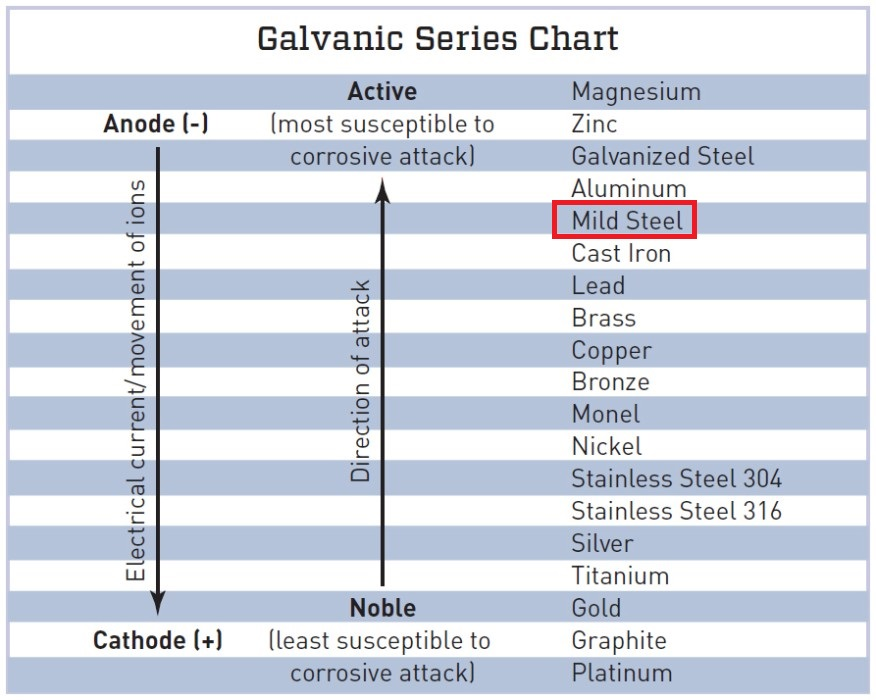
\includegraphics[width=15cm]{PIC/CH02/GAL}
\caption{Galvanic activity (\href{https://www.jlconline.com/how-to/exteriors/separating-galvanic-metals_o}{\url{https://www.jlconline.com/how-to/exteriors/separating-galvanic-metals_o}})}
\end{figure}
\item \textbf{temperature}\\
Metals become brittle under low temperature and ductile/softening under high temperature. It is necessary to provide an environment where the steel does not get too hot nor too cold by, for example:
\begin{itemize}
\item provide adequate ventilation, reduce fuel, e.g., parking structures
\item cover steel surface by using concrete, timber, plaster, chemical foam, mineral fibres, special paints, etc.
\end{itemize}
\begin{figure}[H]
\centering\footnotesize
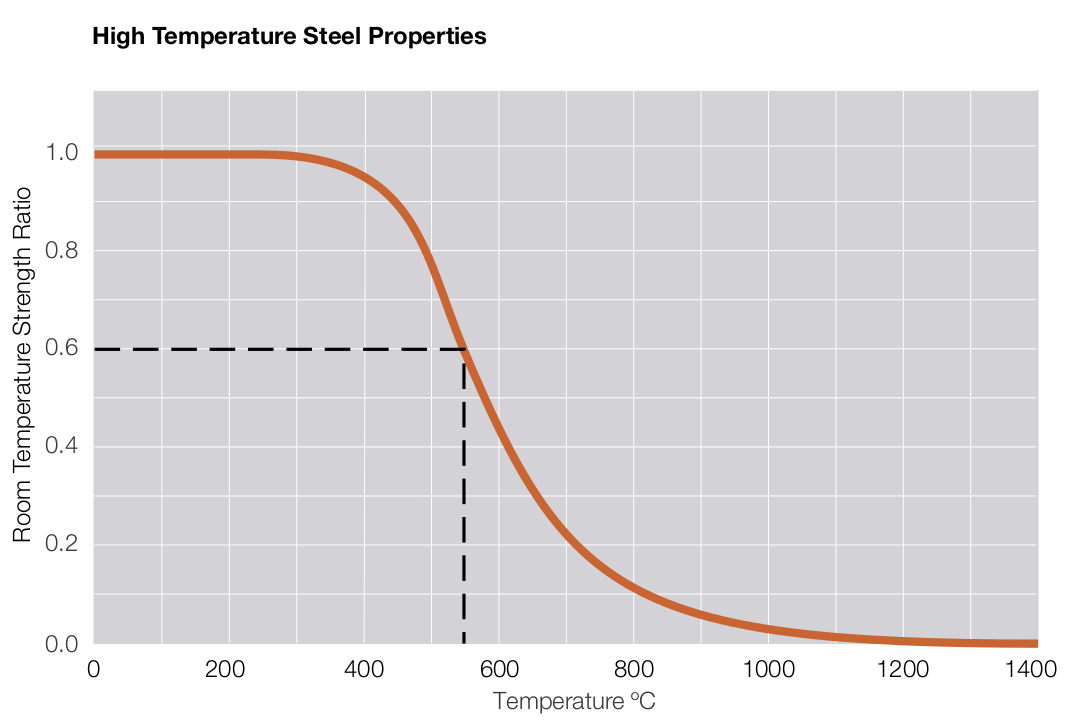
\includegraphics[scale=.4]{PIC/CH02/TEMP}
\caption{Steel strength decreases with temperature \citep{Espinos2015}}
\end{figure}
\item \textbf{residual stress}\\
Residual stresses may occur in steel members/elements as a result of nonuniform cooling of the section. It may occur due to rolling or welding. For the section shown below, it will cool fastest at the extremities, where there is less additional steel to maintain its temperature. Once the extremities cool, they become solid. Then, as the core (away from the extremities) cools, it tries to shorten. As it does this it pulls on the extremities, so that they shorten too. However, as the extremities are solid, they do not shorten. Instead, they become subject to a compressive force as they resist the shortening. Also, the core remains in tension as it is unable to cause the extremities to shorten. Therefore, in general, extremities are in compression, while the core is in tension. Welded sections may have significantly different behaviour.
\begin{figure}[H]
\centering

\footnotesize
\begin{tikzpicture}
\draw[dashed](-3,-.8)rectangle(3,.8);
\draw[dashed](-3,-.1)rectangle(3,.1);
\draw[very thick,fill=cc0066,fill opacity=.6](-3,-.8)rectangle(3,.8);
\node[align=left,anchor=west]at(-8,0){hot --- steel directly from\\furnace};
\draw[very thick,fill=cc0066,fill opacity=.6](3.5,-.8)rectangle++(.2,1.6);
\draw[very thick,fill=cc0066,fill opacity=.6](5.5,-.8)rectangle++(.2,1.6);
\draw[very thick,fill=cc0066,fill opacity=.6](3.7,-.1)rectangle(5.5,.1);
\begin{scope}[yshift=-3cm]
\draw[dashed](-3,-.8)rectangle(3,.8);
\draw[dashed](-3,-.1)rectangle(3,.1);
\draw[very thick](-2.8,-.8)rectangle(2.8,.8);
\draw[fill=cc0066,fill opacity=.6](-2.8,-.3)rectangle(2.8,.3);
\node[align=left,anchor=west]at(-8,0){cooling --- extremities\\cool first, hot centre moves\\with extremities};
\draw[very thick](3.5,-.8)rectangle++(.2,1.6);
\draw[very thick](5.5,-.8)rectangle++(.2,1.6);
\draw[very thick](3.7,-.1)rectangle(5.5,.1);
\draw[very thick,fill=cc0066,fill opacity=.6](3.5,-.3)rectangle++(.2,.6);
\draw[very thick,fill=cc0066,fill opacity=.6](5.5,-.3)rectangle++(.2,.6);
\draw[very thick,fill=cc0066,fill opacity=.6](3.7,-.1)rectangle(4,.1);
\draw[very thick,fill=cc0066,fill opacity=.6](5.2,-.1)rectangle(5.5,.1);
\end{scope}
\begin{scope}[yshift=-6cm]
\draw[dashed](-3,-.8)rectangle(3,.8);
\draw[dashed](-3,-.1)rectangle(3,.1);
\draw[very thick](-2.8,-.8)--++(5.6,0)to[out=90,in=-90]++(-.1,.8)to[out=90,in=-90]++(.1,.8)--++(-5.6,0)to[out=-90,in=90]++(.1,-.8)to[out=-90,in=90]++(-.1,-.8);
\node[align=left,anchor=west]at(-8,0){cooled --- centre cools and\\wants to shorten\\but it is restrained by stiff\\cooled extremities};
\draw[very thick](3.5,-.8)rectangle++(.2,1.6)node[midway,above=8mm]{C}node[midway,below=8mm]{C}node[midway,left=1mm]{T};
\draw[very thick](5.5,-.8)rectangle++(.2,1.6)node[midway,above=8mm]{C}node[midway,below=8mm]{C}node[midway,right=1mm]{T};
\draw[very thick](3.7,-.1)rectangle(5.5,.1)node[midway,above=1mm]{C};
\end{scope}
\node at(0,-8){This puts extremities into compression and central regions into tension.};
\end{tikzpicture}

\caption{Residual stress from cooling member}
\end{figure}

Although the section as whole is in equilibrium, due to residual stresses, some regions are in compression while some in tension. When loaded, the section yields non-uniformly. The tension force displacement curve of a member becomes rounded as the stress approaches the yield value, but the peak tensile strength does not change. However, in the case of compression force, the rounded stress--strain curve implies a lower member axial stiffness. Since the buckling load is related to the stiffness, the compressive strength can decrease. This affects members of intermediate slenderness (as stocky members do not buckle, and slender members buckle before the residual stresses affect the response).
\begin{figure}[H]
\centering\footnotesize
\begin{tikzpicture}[>=latex]
\begin{axis}[
width=10cm,
height=6cm,
xtick=\empty,
ytick=\empty,
axis x line=center,
axis y line=center,
xlabel={section deformation},
ylabel={section force},
xlabel style={below},
ylabel style={right},
xmin=0,xmax=4.5,ymin=0,ymax=2]
\addplot[line width=.8mm,mark=none]coordinates{
(0,0)
(.3,1.5)
(3.5,1.5)
}node[align=left,above,pos=1]{ideal response\\without residual stress};
\addplot[line width=.8mm,color=cc0066,domain=0:3.5,samples=100]{1.5*(x/.3/(1+(x/.3)^2)^0.5)}node[align=left,below,pos=1]{response with\\residual stress};
\end{axis}
\end{tikzpicture}
\caption{Stress--strain curve considering residual stress}
\end{figure}

Depending on different geometries/configurations, different residual stress patterns may appear as shown in the following figure.
\begin{figure}[H]
\centering\footnotesize
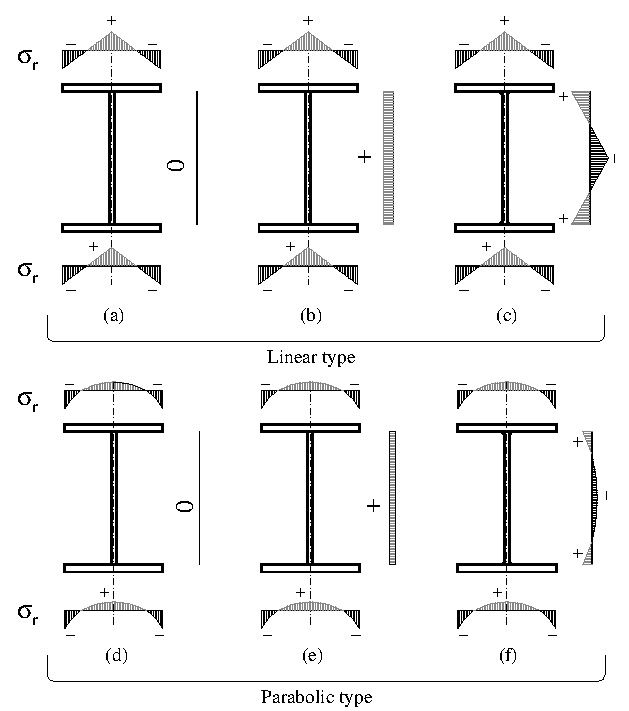
\includegraphics{PIC/CH02/RS2}
\caption{Residual stress patterns of hot-rolled sections (\href{https://www.lajss.org/index.php/LAJSS/article/view/176}{\url{https://www.lajss.org/index.php/LAJSS/article/view/176}})}
\end{figure}
\item \textbf{steel detailing}\\
Rapid changes in cross section shape can cause stress concentrations.
\begin{figure}[H]
\centering\footnotesize
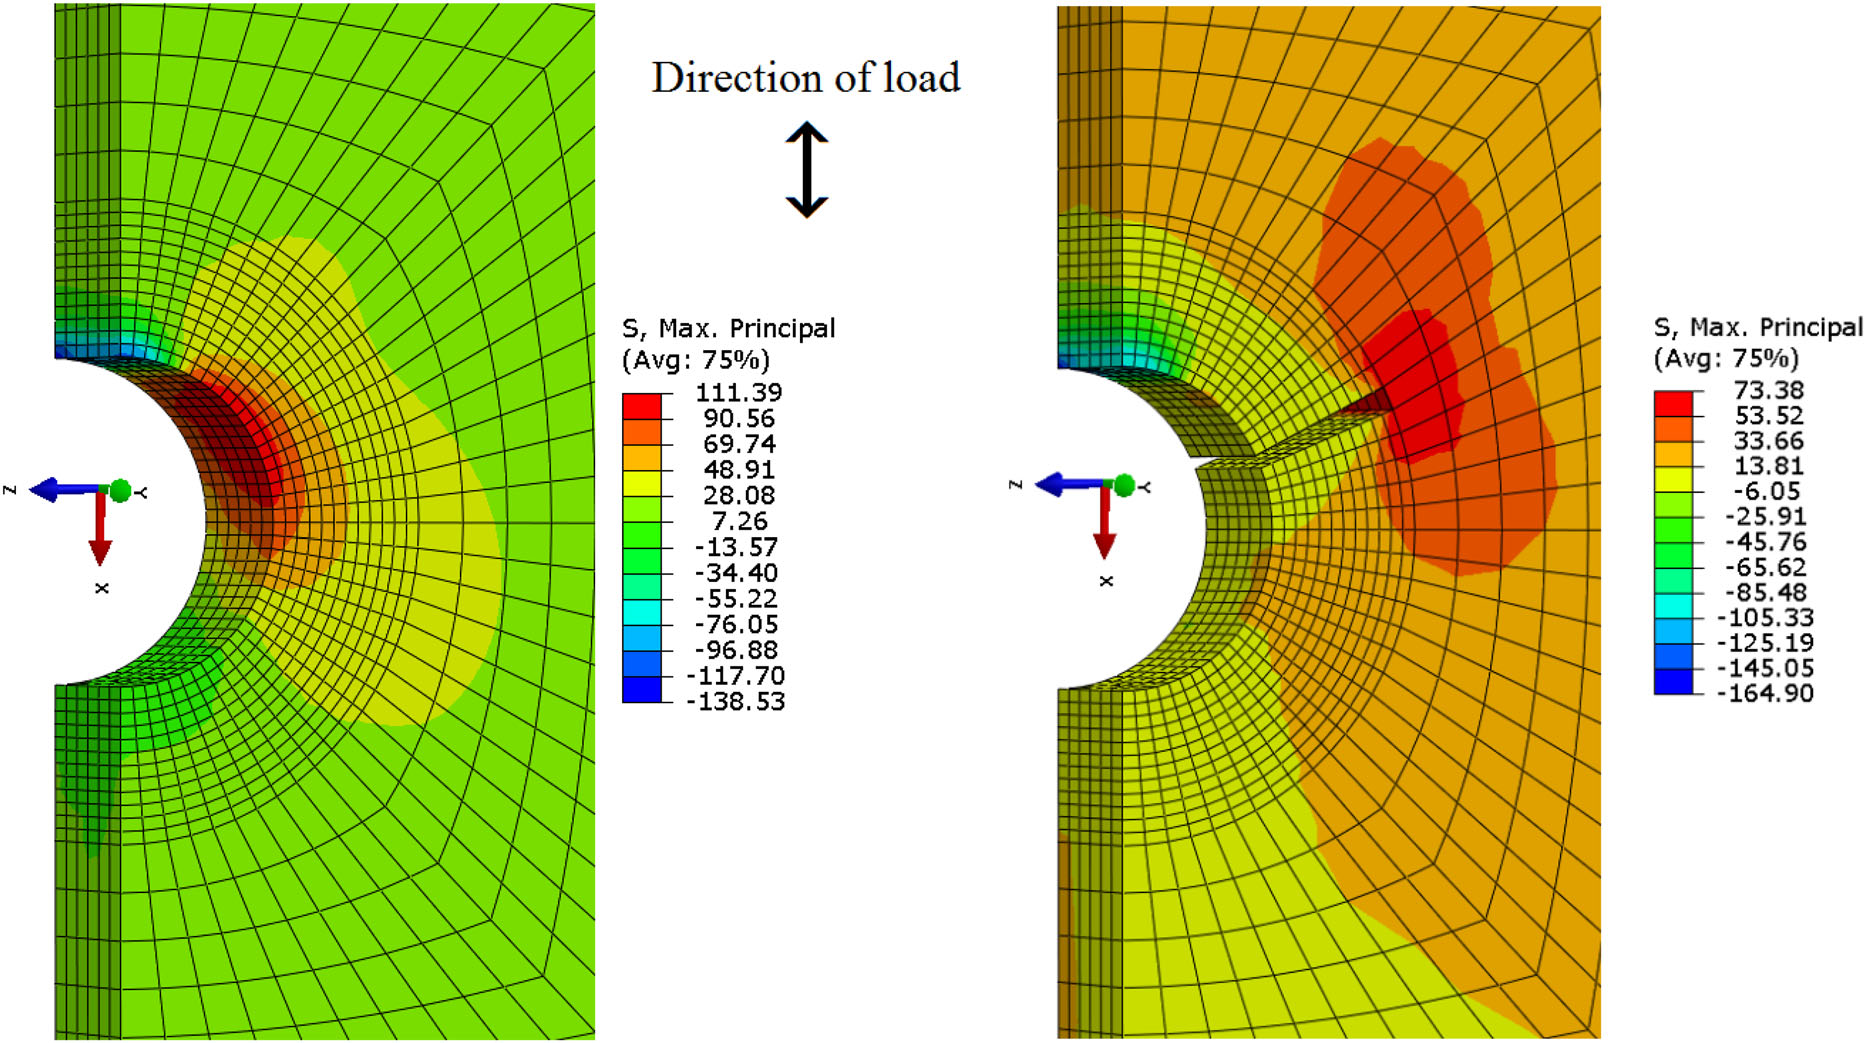
\includegraphics[width=12cm]{PIC/CH02/SC}
\caption{Stress concentration due to sharp change of geometry \citep{Katsivalis2018}}
\end{figure}
\begin{figure}[H]
\centering\footnotesize
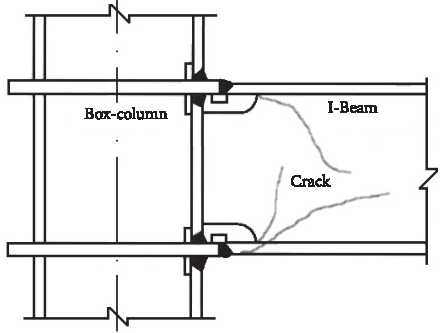
\includegraphics[width=8cm]{PIC/CH02/SD}
\caption{Crack in connections \citep{Qu2017}}
\end{figure}
\item \textbf{steel quality}\\
Poor quality steel is more likely to be brittle. Brittle behaviour is possible as a result of:
\begin{itemize}
\item large dimension ($t>\SI{20}{\mm}$)
\item defects (inclusions, air pockets, etc.) in steel
\item weak lamellar bonds
\end{itemize}
\begin{figure}[H]
\centering\footnotesize
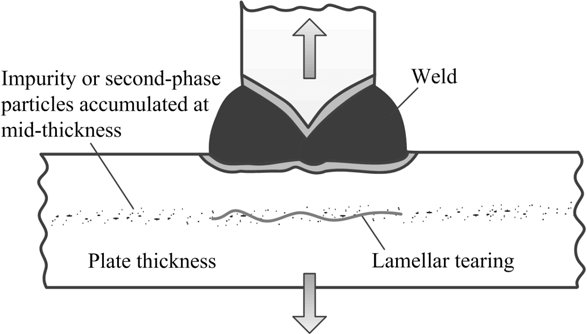
\includegraphics[width=8cm]{PIC/CH02/LT}
\caption{Illustration of lamellar tearing in thick steel plates (\href{http://sainsmechanical.blogspot.com/2011/12/hot-working-of-metals.html}{\url{http://sainsmechanical.blogspot.com/2011/12/hot-working-of-metals.html}})}
\end{figure}
\begin{figure}[H]
\centering\footnotesize
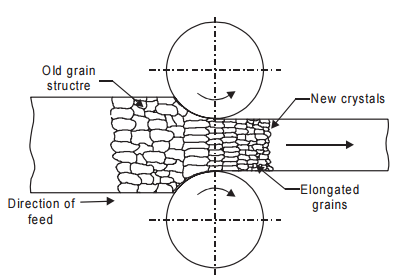
\includegraphics[width=7cm]{PIC/CH02/HW}
\caption{Gain reshaped due to rolling}
\end{figure}
\item \textbf{cold working}\\
Possibility of fracture is increased after cold working, thus one shall be careful if reusing steels.
\begin{figure}[H]
\centering\footnotesize
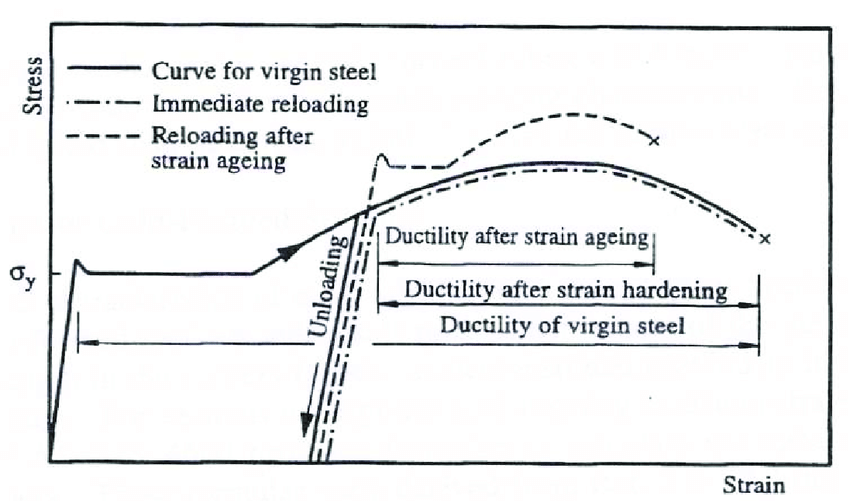
\includegraphics[width=10cm]{PIC/CH02/SH}
\caption{Strain hardening by cold working}
\end{figure}
\item \textbf{strain ageing}\\
Strain aged steel is stronger but more brittle.

Steel is initially loaded to point A for some time then unloaded. When reloaded, it can reach point B and follow the corresponding path as shown in the figure.
\begin{figure}[H]
\centering\footnotesize
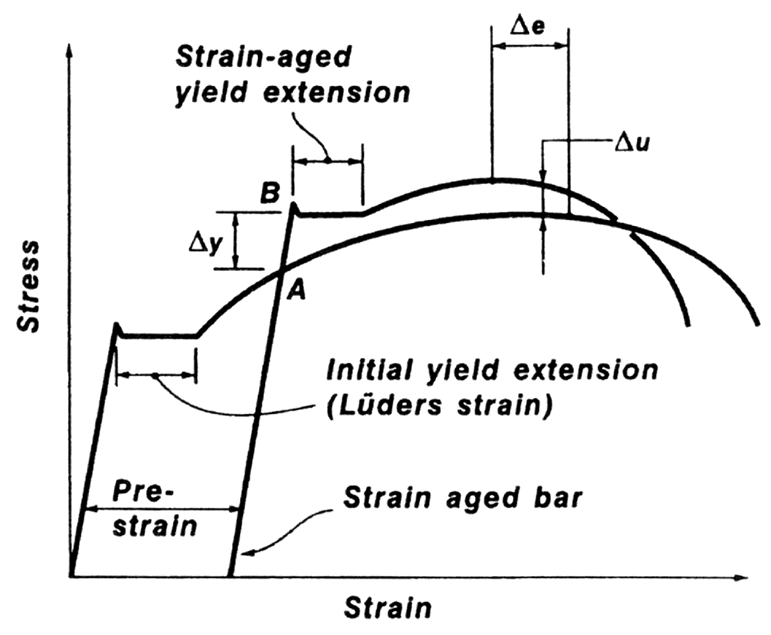
\includegraphics[width=7cm]{PIC/CH02/AGEING}
\caption{Strain ageing}
\end{figure}
\item \textbf{repeated loading}\\
As the material sustains many elastic load reversals it may lead to brittle failure characterised by \href{https://en.wikipedia.org/wiki/Fatigue_(material)}{fatigue}. Fatigue fracture is dependent on magnitude of stress reversal as well as the number of cycles applied. It is most significant when there are sharp discontinuities in the material shape. It is not usually a concern in buildings, but can be a problem due to traffic on bridges.
\begin{figure}[H]
\centering
\footnotesize
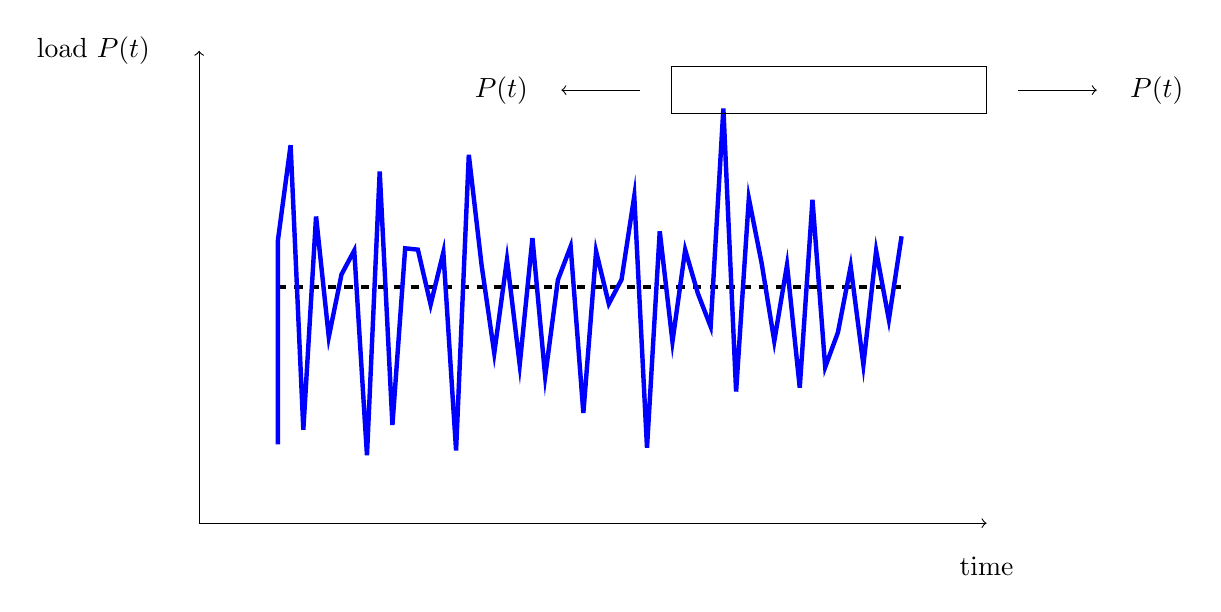
\begin{tikzpicture}[declare function={excitation(\t,\w)=sin(\t*\w);noise=rnd-.5;source(\t)=excitation(\t,20)+noise;filter(\t)=1-abs(sin(mod(\t,50)));speech(\t)=1+source(\t)*filter(\t);}]
\draw[->](0,0)--(10,0)node[below=3mm]{time};
\draw[->](0,0)--(0,6)node[left=5mm]{load $P(t)$};
\draw[dashed,very thick](1,3)--(9,3);
\begin{scope}[xshift=1cm,yshift=1cm]
\draw[blue,ultra thick,x=.022cm,y=2cm](0,0)--plot[domain=0:360,samples=50] (\x,{speech(\x)});
\end{scope}
\begin{scope}[xshift=8cm,yshift=5.5cm]
\draw(-2,-.3)rectangle(2,.3);
\draw[->](2.4,0)--++(1,0)node[right=3mm]{$P(t)$};
\draw[->](-2.4,0)--++(-1,0)node[left=3mm]{$P(t)$};
\end{scope}
\end{tikzpicture}

\caption{Cyclic loads}
\end{figure}
\begin{figure}[H]
\centering\footnotesize
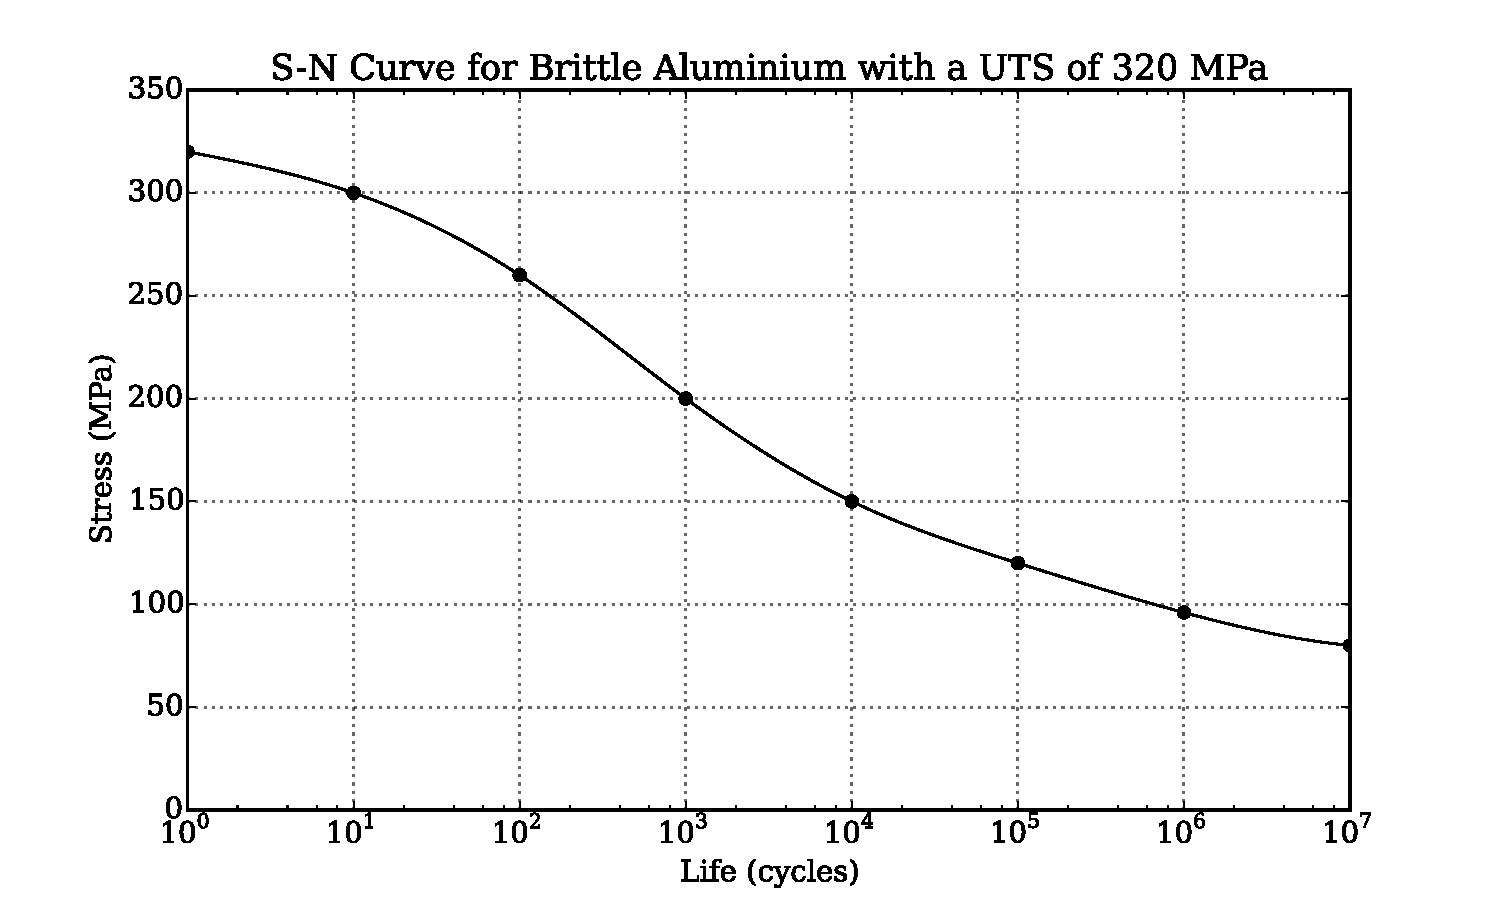
\includegraphics[width=12cm]{PIC/CH02/FATIGUE}
\caption{Stress--life curve for a brittle aluminium (\href{https://upload.wikimedia.org/wikipedia/commons/d/d2/BrittleAluminium320MPa_S-N_Curve.svg}{\url{https://upload.wikimedia.org/wikipedia/commons/d/d2/BrittleAluminium320MPa_S-N_Curve.svg}})}
\end{figure}
\item \textbf{impact loading}\\
High speed loading can lead to more brittle failure. This is often indicated by \href{https://www.youtube.com/watch?v=tpGhqQvftAo}{Charpy V-notch}\footnote{https://www.youtube.com/watch?v=tpGhqQvftAo} test.

High impact resistance is important for structures subject to earthquake shaking.

The mass is released from specified height. The angle $\theta$ the mass moves to after breaking specimen is recorded as a measure of ductility. Often low $\theta$, indicating more energy is absorbed by the specimen, is desired.
\begin{figure}[H]
\centering
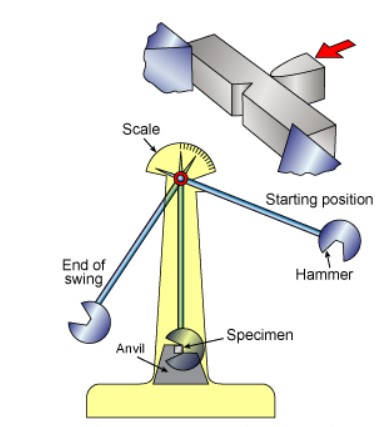
\includegraphics[scale=.6]{PIC/CH02/CIT}
\caption{Charpy V-notch test apparatus (\href{https://www.totalmateria.com/page.aspx?ID=CheckArticle\&site=kts\&NM=534}{\url{https://www.totalmateria.com/page.aspx?ID=CheckArticle&site=kts&NM=534}})}
\end{figure}
\item \textbf{triaxial loading}\\
Depending on loading direction, triaxial loading conditions may lead to an increase or decrease in strength. An increase in strength is generally associated with a decrease in ductility.
\begin{figure}[H]
\centering\footnotesize
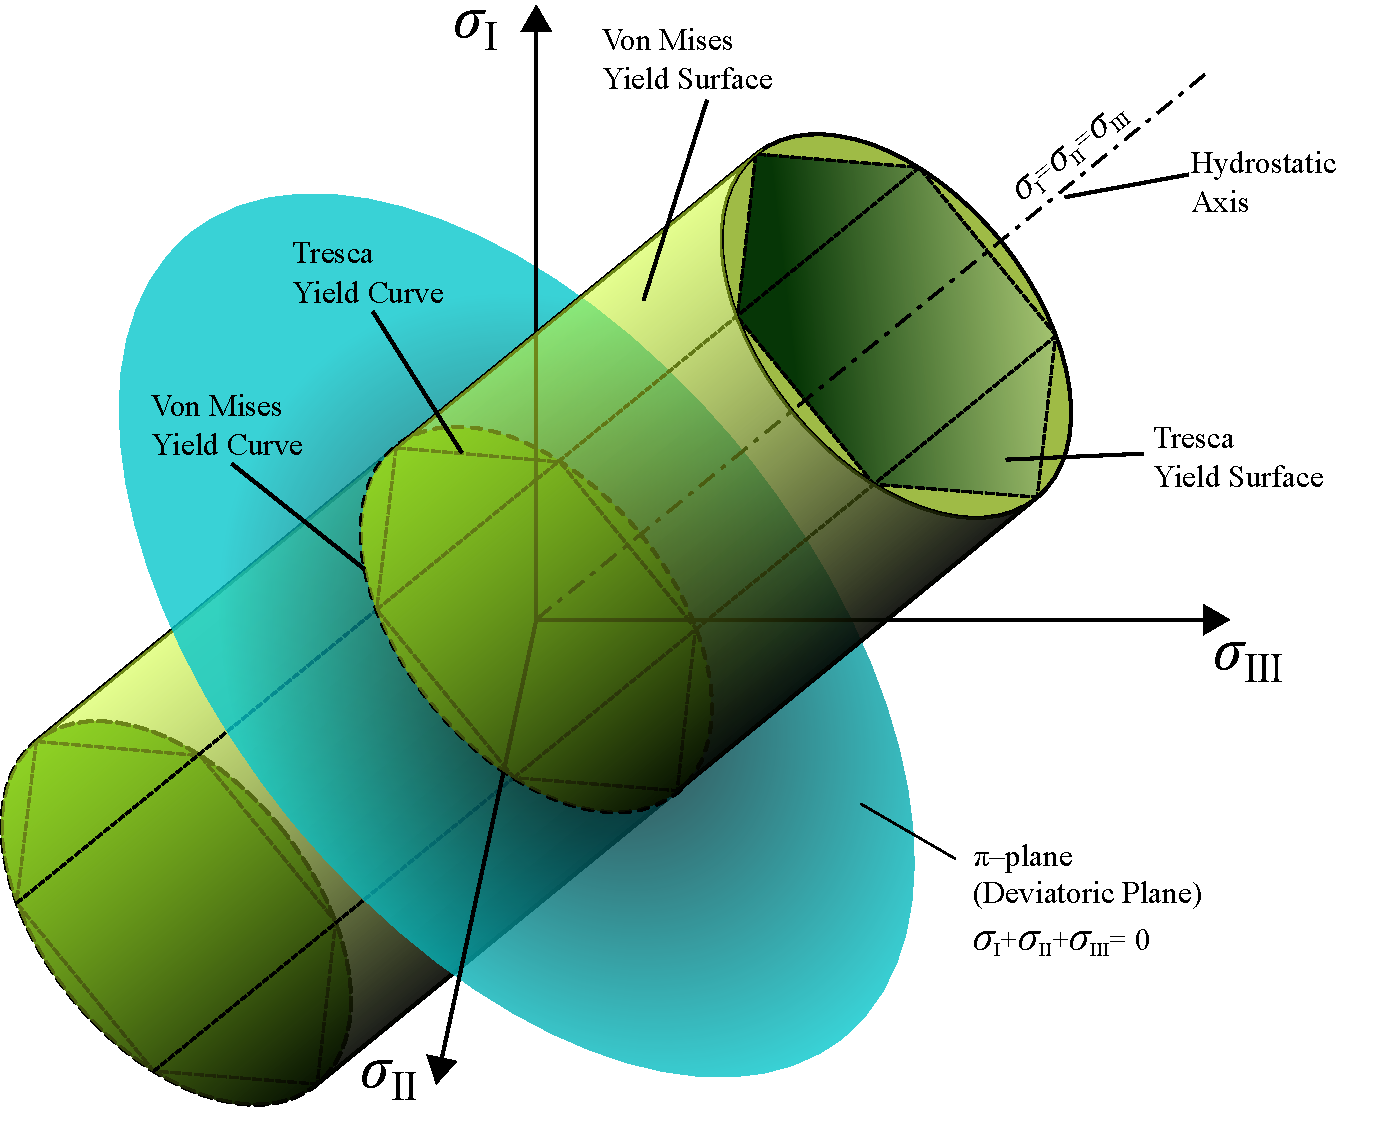
\includegraphics[width=12cm]{PIC/CH02/MISES}
\caption{von Mises yielding criterion (\href{https://upload.wikimedia.org/wikipedia/commons/c/cc/Yield_surfaces.svg}{\url{https://upload.wikimedia.org/wikipedia/commons/c/cc/Yield_surfaces.svg}})}
\end{figure}
\end{itemize}
